%%
%% This is file `cescgsmpl.tex',
%% generated with the docstrip utility.
%%
%% The original source files were:
%%
%% cescg.dtx  (with options: `sample')
%% 
%% IMPORTANT NOTICE:
%% 
%% For the copyright see the source file.
%% 
%% Any modified versions of this file must be renamed
%% with new filenames distinct from cescgsmpl.tex.
%% 
%% For distribution of the original source see the terms
%% for copying and modification in the file cescg.dtx.
%% 
%% This generated file may be distributed as long as the
%% original source files, as listed above, are part of the
%% same distribution. (The sources need not necessarily be
%% in the same archive or directory.)
%% Copyright (c) 1999, 2005
%%               Institute of Computer Graphics and Algorithms
%%               TU Vienna, Austria
%% Based on the LaTeX2e document class SCCG
%% Copyright (C) 1999 Pavel Chalmoviansky
%%                    Katedra geometrie
%%                    Faculty of Mathematics and Physics
%%                    Comenius University, Bratislava
%%                    chalmo@fmph.uniba.sk
%%
%% This file is distributed in the hope that it will be useful,
%% but WITHOUT ANY WARRANTY; without even the implied warranty of
%% MERCHANTABILITY or FITNESS FOR A PARTICULAR PURPOSE.
%%
%% \CharacterTable
%%  {Upper-case    \A\B\C\D\E\F\G\H\I\J\K\L\M\N\O\P\Q\R\S\T\U\V\W\X\Y\Z
%%   Lower-case    \a\b\c\d\e\f\g\h\i\j\k\l\m\n\o\p\q\r\s\t\u\v\w\x\y\z
%%   Digits        \0\1\2\3\4\5\6\7\8\9
%%   Exclamation   \!     Double quote  \"     Hash (number) \#
%%   Dollar        \$     Percent       \%     Ampersand     \&
%%   Acute accent  \'     Left paren    \(     Right paren   \)
%%   Asterisk      \*     Plus          \+     Comma         \,
%%   Minus         \-     Point         \.     Solidus       \/
%%   Colon         \:     Semicolon     \;     Less than     \<
%%   Equals        \=     Greater than  \>     Question mark \?
%%   Commercial at \@     Left bracket  \[     Backslash     \\
%%   Right bracket \]     Circumflex    \^     Underscore    \_
%%   Grave accent  \`     Left brace    \{     Vertical bar  \|
%%   Right brace   \}     Tilde         \~}
%%
\ProvidesFile{cescgsmpl.tex}
            [2005/11/29 v0.1.4
 CESCG proceedings sample file]
 %%% The document class command loads the CESCG class and sets the basic
 %%%  options.  See the user's guide for more options and their meaning.


\documentclass{cescg}[2005/11/12] % Use this for your submission and the final paper
 %%% Use e.g. this package to include figures via \includegraphics[options]{filename}.
 %%% If you don't have it in your latex installation, complain to your
 %%% sysadmin that he's not doing his job.
\usepackage{graphicx}
 %%% The following packages are somewhat system and installation dependent, and may not work
 %%% on some systems.
 %%% If you use pdfLaTeX on Windows (part of MiKTeX), you may use package epstopdf to automatically
 %%% convert eps files to pdf. Use this line:
 %\usepackage{epstopdf}
 %%% Linux users may have to call epstopdf on the command line or configure a Makefile appropriately.

 %%% If you know how to create bounding boxes for png and jpg files, you can uncomment this
 %%% to include png files etc. directly.
 %%% For example bmeps -b myfigure.png >myfigure.bb will do the trick in Windows.
 %%% Also, dvips needs the option "-I c3r8f" to be able to convert the bitmaps.
 %%% See the bmeps faq for more info: http://bmeps.sourceforge.net/faq.html
 %\ifx\pdfoutput\undefined \DeclareGraphicsExtensions{.eps,.png,.gif,.jpg} \fi

 %%% Now we set the fields for the title block and cover sheet
 %%% See the user's guide for more information on these items

 %% Title, author(s), and affiliation
 %%  Note that we have included both individual affiliations for each author
 %%   within the author block, as well as a common affiliation.  Only one
 %%   of these is necessary.
 %%  Footnotes to items in the title block should be created with the \thanks
 %%   command.
\title{Rapid Modeling of Geology}
\author{Morten Bendiksen\thanks{morten.bendiksen@gmail.com}}
\supervisor{Endre M. Lidal\thanks{endre.lidal@gmail.com}, Ivan Viola\thanks{ivan.viola@uib.no}} % TODO add emails
\affiliation{Institute of Informatics\\
             University of Bergen}

 %% Keywords of paper
\keywords{Rapid Modeling, SBIM, Geology}
 %%% Begin the paper
\begin{document}

 %%% Create the title block
\maketitle

 %%% The abstract
\begin{abstract}
 Drawing three dimensional models of geological phenomena is today a process requiring training in specific programs that can be very time consuming. For illustration and communication of geological concepts, geologists therefore often limit themselves to drawing on paper or to two dimensional drawing applications.

I propose an approach for making rapid geologic illustrations in 3D. The novel idea for the approach consists of sketch based input on a cube in order to create a layered geological structure. Further details can be added to the layers by sketching geological concepts such as rivers, mountains and valleys. Sedimentary deposits can be created through a procedural modeling approach that employs a volume preserving diffusion algorithm to simulate the flow of depositional material on top of the terrain. Awareness of the geologic domain enables a sparse amount of input strokes to be interpreted into geological structures.

Results show that the proposed approach can be used with success to model geological layers. Compared with a 2D sketch, the creation of a 3D geometry on a computer gives advantages such as perspective control, ease of making changes to the model, etc. The approach shows great promise and can be useful in many situations. A program based on the proposed approach could become a standard way for geologists to draw their illustrations.
\end{abstract}

 %%% Keywords

\keywordlist

 %%% The main text
\section{Introduction}

\begin{figure}
 \centering
 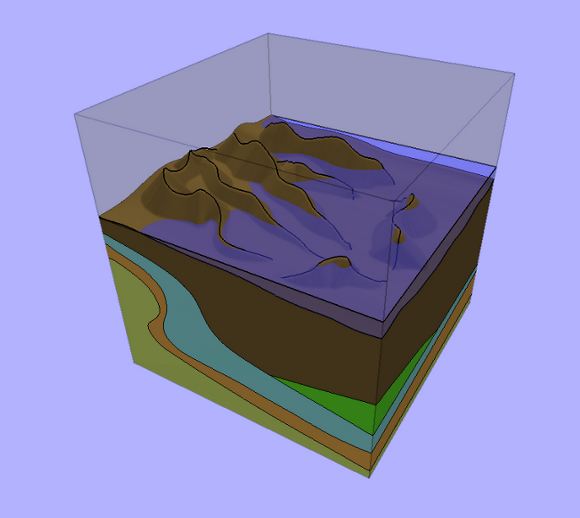
\includegraphics[width=0.7\linewidth]{approachSketch.png}
 % TODO insert reference
 \caption{A typical sketch made with the proposed approach. }
 \label{fig:approachSketch}
\end{figure}

% 
% \begin{figure}[b]
%  \centering
%  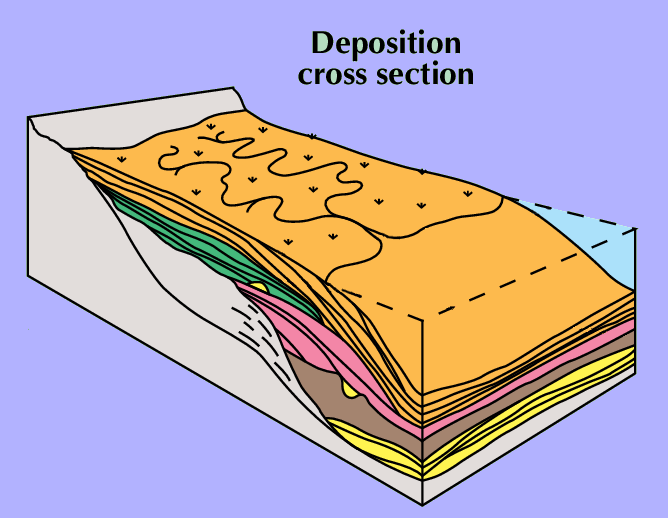
\includegraphics[width=0.7\linewidth]{strataSketch.png}
%  % TODO insert reference
%  \caption{A typical sketch from a earth science paper. }
%  \label{fig:strataSketch}
% \end{figure}
It is a common practice to make sketched geological models by hand on either paper or computer. These sketches are used in both professional and educational settings, and facilitate communication and understanding. Geologic phenomena are four dimensional in nature since they occur over time in the three spatial dimensions. There are many techniques and standards for illustrating these phenomena in a two dimensional drawing. One can for example sketch three dimensional phenomena by using perspective drawing techniques, but the model is still confined to the 2D nature of the medium. These techniques and standards can also be limiting  as they require significant time and training to master and understand. Before I started working on this project a problem was identified; there did not exist any tools aimed at helping geologists sketch 3D models for illustration purposes. On the computer it is already possible to make 3D models in traditional modeling approaches. However, existing tools are often complex, aimed 
at creating advanced and detailed models, and usually requires training to understand and use. It is from this background that the goal of this project was formed. 


The goal is to enable the rapid creation of 3D models of geologic structures by creating an approach that lets geologists quickly specify input in an intuitive way that is easy to learn. The model will be used for illustrative purposes to facilitate communication between geologists by letting them create sketched models quicker, help lecturers explain concepts to students by creating models that can be changed interactively, and reduce the need for artistic skills and long training for students to master illustration techniques. The study of sedimentary layer structures and the processes that deform such layers are perhaps the fields of study that has resulted in the most knowledge about the history of the Earth. I concentrate most effort around the creation of rapid modeling techniques for geological layer structures. The aim is to create an approach for the creation of such structures.

\section{Background}
The geologic understanding for this project was gained from reading the book ``Geologi, Stein, mineraler, fossiler og olje'', by Haakon Fossen \cite{fossen2008geologi}. For reference and technical background in the field of computer graphics the book ``Real Time Rendering'' \cite{moller2008real} has been used.  The book ``Curves and surfaces for CAGD: a practical guide'' \cite{farin2001curves} was used to understand curve and surface theory. 

Geology is a complex science with many subfields. Geomorphology is the study of landforms and the processes that shape the surface of the Earth. Sedimentology is about how particles are transported, where they are deposited and how they are compressed into rock. Structural geology is the study of how the rock layers and crust is deformed by various movements. Tectonics is closely related to Structural geology and describes the movement of Earth plates and how that causes the formation of mountain ranges and basins. There are many other fields, but these are the ones of most relevance to my research.

In geology, models are used for understanding and communicating about phenomena relating to the structure of the Earth and how it changes over time. Traditional CAD systems have several problems when used to make geological models (Turner et al. \cite{turner2006challenges}, Kelk and Challen \cite{kelk1992experiments}). The gOcad tool decscribed by Mallet \cite{mallet1992gocad}, however, has been developed to make a CAD approach for geomodeling, by basing the modeling on a new interpolation method called ``Discrete Smooth Interpolation''. The geometry is defined by bridging together a set of nodes with a location is 3D space and with physical properties attached to these nodes.

A realistic geological scenario will follow certain constraints.  Caumron et al. \cite{caumon2009surface} gives rules for modeling that define boundaries between layers. For example, geological objects have a spacial continuity such that abrupt changes of normal orientation are not common. This is relevant for the creation of layers in the approach I propose, as it allows the use of smooth curves to represent layers. 

For creating layers for geologic modeling, interpolation methods are important. The main interpolation methods are the B-Spline method, inverse distance method, Kriging method, and discrete smooth interpolation method \cite{mallet1992discrete, mallet1997discrete}. Interpolation methods are interesting in regards to the approach I propose as they might be used to interpolate horizons from the sketched curves for horizon creation. 

Natali et al. explores different modeling techniques in their recent survey paper \cite{natali2013modeling}. They show how geological modeling trends are approaching modeling methods that have been developed in computer graphics and give an in-depth description of selected methods that can be applied for geological modeling. 

Often geologists are creating models based on an interpretation of available data. Approaches that aim at making the interpretation process easier and quicker have emerged in recent years. Patel et al. describe techniques for rapid horizon extraction from seismic data in both 2D \cite{patel2008seismic} and 3D \cite{patel2010seismic}. Amorim et al. \cite{amorim2012sketch} have an interesting approach that allows sketching directly over the raw seismic reflection volume and its derived data to help build the structural model of the subsurface. This helps the expert in interpreting and and building a structural framework for a reservoir by using a sketch-based input for helping in the interpretation process. Petrel \cite{petrel} is an example of a commercial program for geologic modeling that is in use. Most of such existing tools rely on an intensive work flow,and up to a year is spent on developing such models. Recently a need for rapid developments of geologic prospects have been identified.

 Procedural generation is a standard way to generate terrains. This usually happens in one of three ways: fractal landscape modeling, physical erosion simulation and synthesis of terrain from images or sample terrain. Before Olsen \cite{olsen2004realtime} fractal noise was mostly used to create terrain surfaces, because of computer limitations on simulating erosion processes. Olsen proposed a synthesized fractal terrain and applies an erosion algorithm on that. The representation is a 2D height-map. Hnaidi et al. \cite{hnaidi2010feature} generate terrain that is constrained by a set of curves that characterize the features of the landscape. The ability to make realistic looking landscapes could be interesting in a rapid sketching tool, as the generated landscape is constrained by curves that could be input by sketching.
 
% \begin{figure}
%  \centering
%  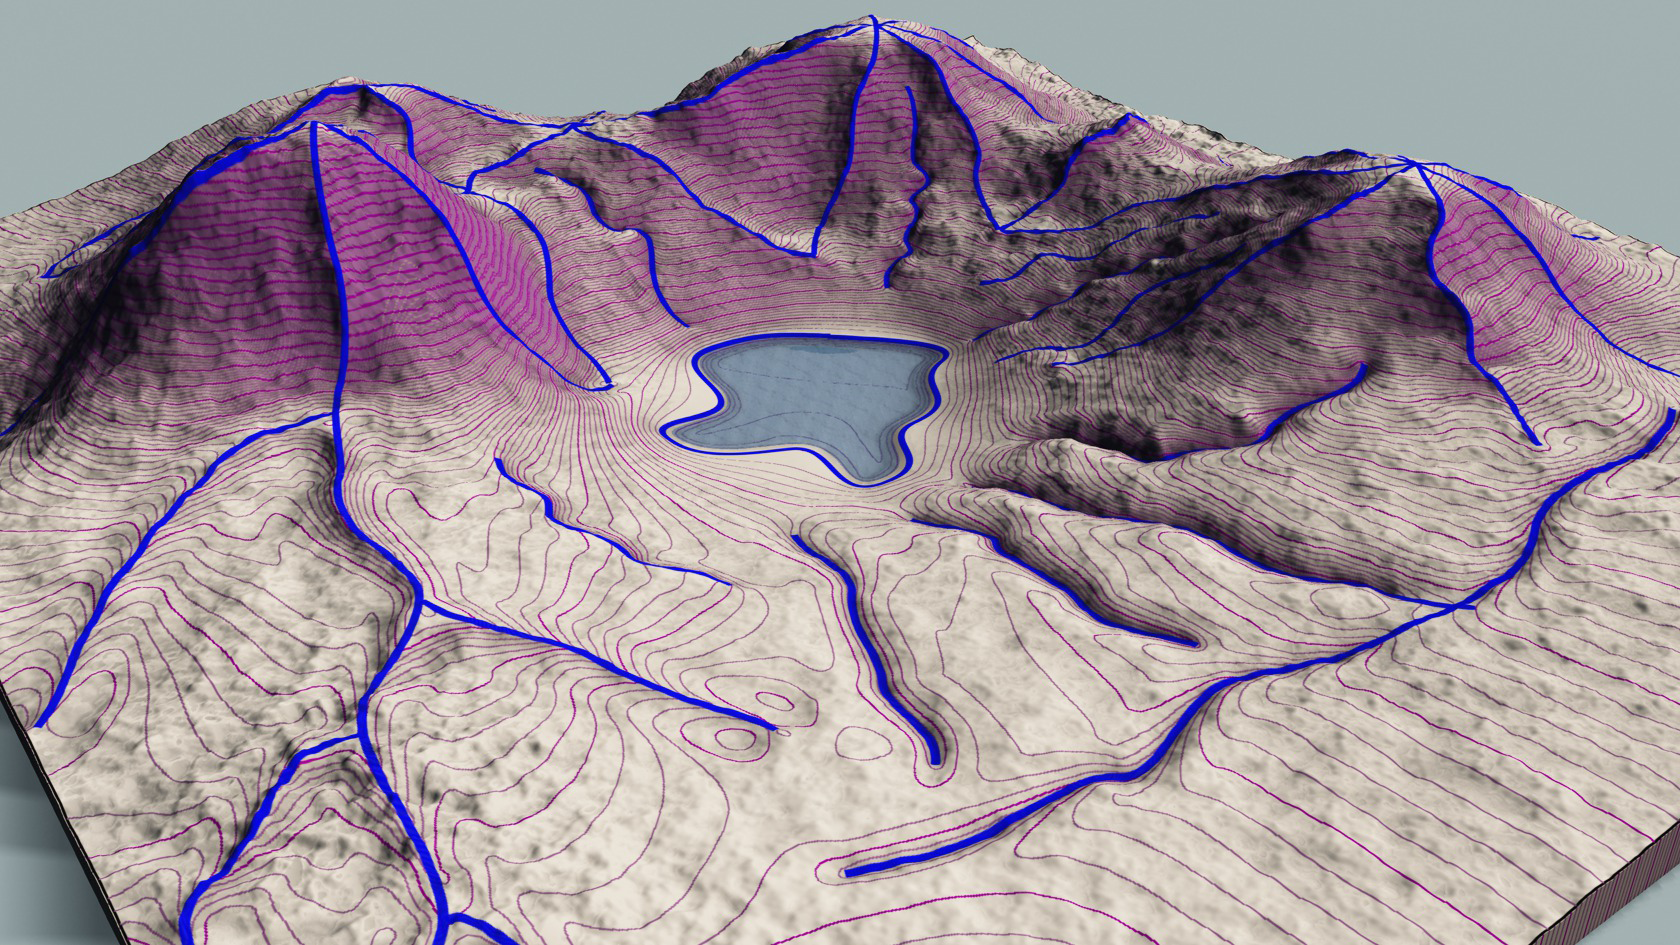
\includegraphics[width=0.5\linewidth]{../thesis/related/hnaidi.png}
%  \caption{Terrain generation by Hnaidi et al. \cite{hnaidi2010feature}. }
%  \label{fig:hnaidi}
% \end{figure}

 A method for eroding terrain is described by Benes et al. \cite{benes2001layered} where a concise voxel representation is created and then eroded by thermal weathering simulation. The representation allows for caves and hole structures. The same authors also propose a method for procedural modeling of terrain by hydraulic erosion \cite{benevs2002visual}. Stava et al. \cite{vst2008interactive} employ an interactive physics based hydraulic erosion. The user interacts during the generation of the terrain. These erosion techniques could be applied in the approach I propose as a way to make more realistic horizon surfaces. Erosion could also be used to simulate material transportation and deposits creation, rivers, etc.
 
 Peytavie et al. \cite{peytavie2009procedural} propose a way to model and render rock piles and stones which are found in most landscapes without any computationally demanding physically-based simulation. Peytavie et al. also have proposed a framework for representing complex terrains with such features as overhangs, arches and caves and including different materials such as sand and rocks \cite{peytavie2009arches}. This is done by a discrete volumetric representation with different kinds of material and an implicit representation for the modelling and reconstruction of the model.

% \begin{figure}
%  \centering
%  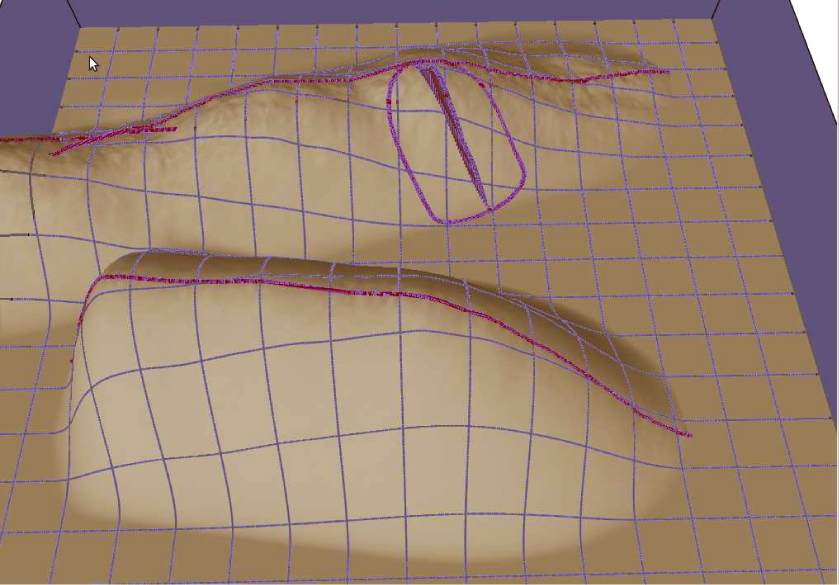
\includegraphics[width=0.4\linewidth]{../thesis/related/tasse1.png}
%  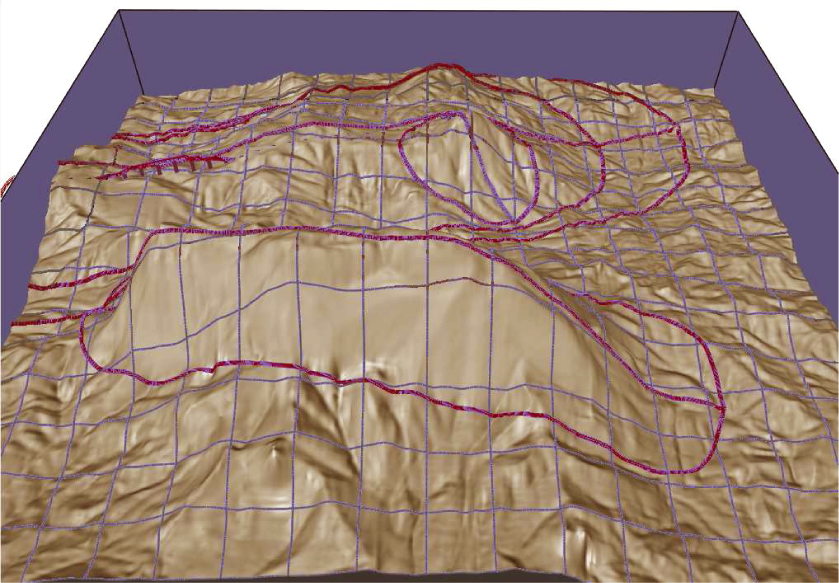
\includegraphics[width=0.4\linewidth]{../thesis/related/tasse2.png}
%  \caption{The terrain syntesis proposed by Tasse et al. \cite{tasse2012enhanced}. Left: user sketched curves. Right: final result. }
%  \label{fig:tasse}
% \end{figure}

Tasse et al. \cite{tasse2012enhanced} propose a texture-based terrain synthesis framework controllable by
a terrain sketching interface. They enhance the realism of the generated landscapes by using a novel patch merging
method that reduces boundary artifacts caused by overlapping terrain patches. The high computational cost of texture
synthesis is reduced with a parallel implementation on graphics hardware. This approach could also prove useful to create more realistic surfaces.

Natali et al. \cite{natalirapid} describe an approach where the user sketches the boundaries of geological layers. Then the user can sketch folding and faulting operations, and thus create many different scenarios. The input in this approach is restricted to making conceptually 2D sketches, allthough the visualization is in 3D. Projecting drawings on the 3D structure can however give some more information and context to the 3D geometry. The techniques for texturing and painting that they describe makes their sketches carry a lot of expressive power of the internal structure of specific layers. As far as I know, this is the only sketch based approach to modeling subsurface geological layers in 3D without measured data other than the one described in this paper. However, Lidal et al. \cite{lidal2012geological} present Geological Storytelling, an approach for rapid and expressive geomodeling of a multitude of model variations in 2D over time. 

\begin{figure}
 
 \centering
    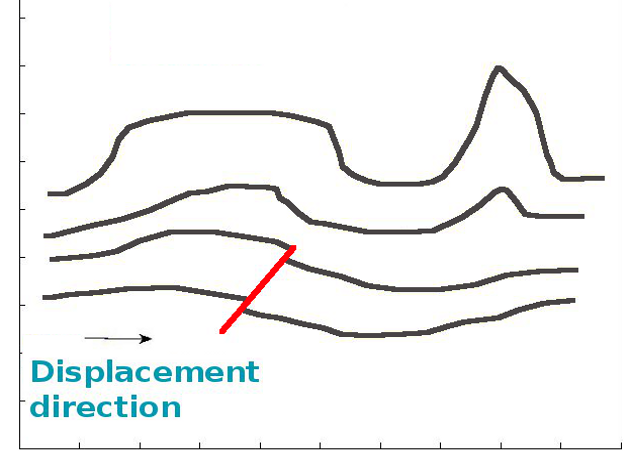
\includegraphics[width=0.3\linewidth]{../thesis/related/natali1.png}
    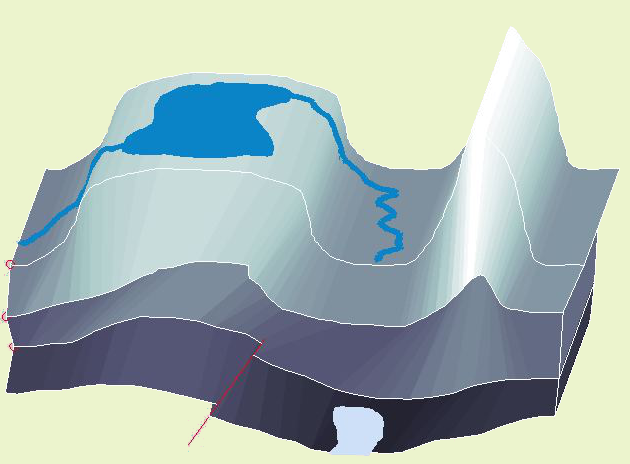
\includegraphics[width=0.3\linewidth]{../thesis/related/natali2.png}
    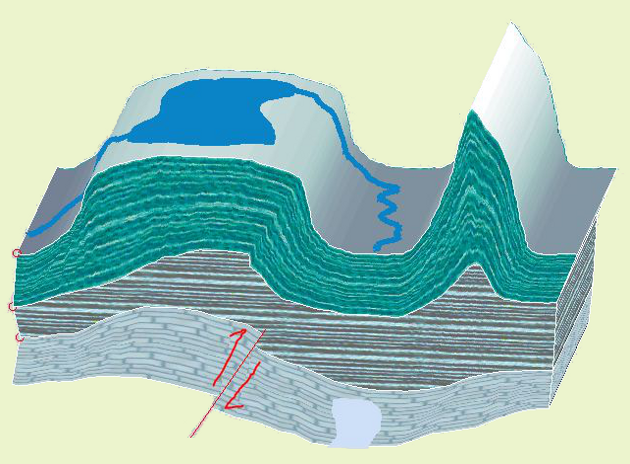
\includegraphics[width=0.3\linewidth]{../thesis/related/natali3.png}
  \caption{The proposed interface by Natali et al. \cite{natalirapid}.  }
  \label{fig:nataliRapid}
\end{figure}


Cockett's Visual Geology \cite{Cockett:Online} and Jessell's Noddy \cite{jessell1981noddy} are two geologic modeling tools designed for educational purposes that allow rapid building of geological layer structures by user input of parameters.

% \begin{figure}
% \centering
%  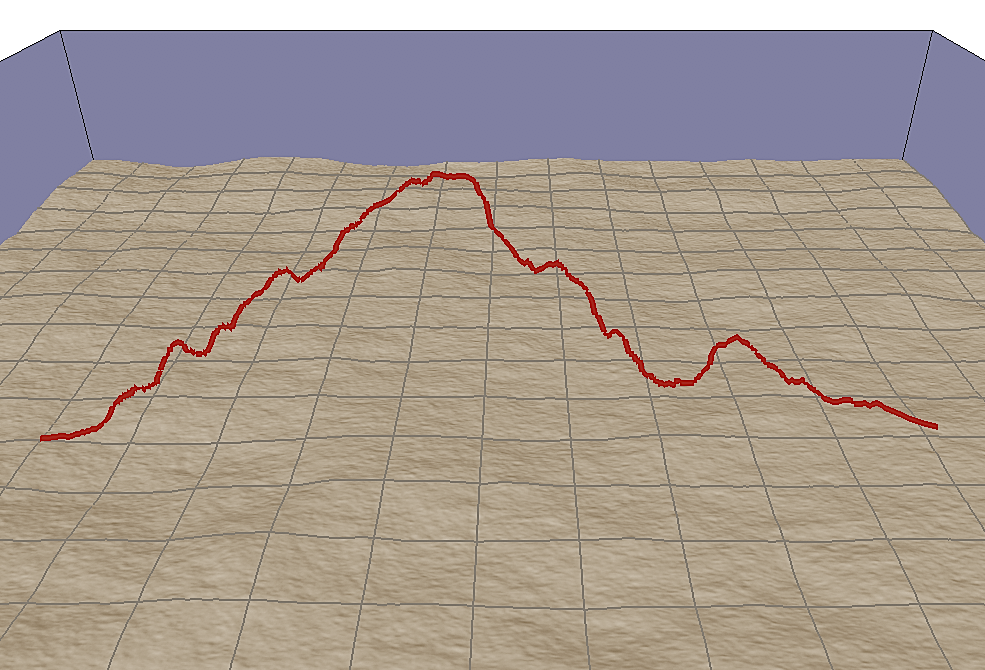
\includegraphics[width=0.4\linewidth]{../thesis/related/img-001.png}
%  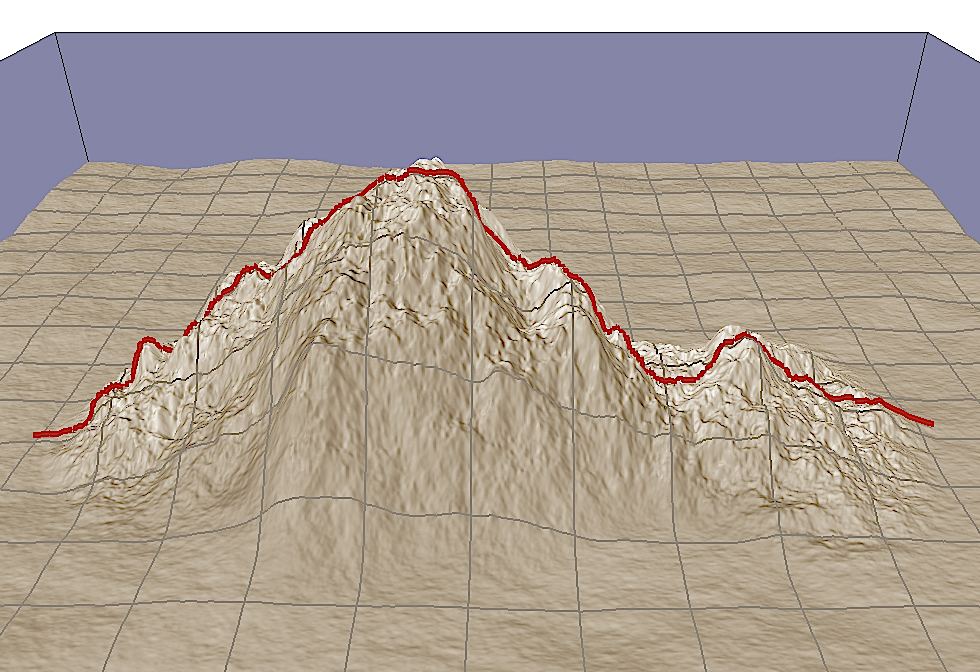
\includegraphics[width=0.4\linewidth]{../thesis/related/img-002.png}
%  \caption{The terrain sketching approach from Gain et al. \cite{Gain:2009:TS:1507149.1507155}. }
%  \label{fig:gain}
% \end{figure}

Harold is an early example of a sketch based system that incorporates methods for sketching terrain, made by Cohen et al. \cite{cohen2000harold}. In Harold, the user can sketch hills on the terrain by simple strokes that start and end on the terrain. The terrain is then warped to try and match the stroke. Watanabe et al.  \cite{Watanabe:2004:SIT:1186415.1186500} made a further development of this, where the shape of the stroke also influences the width of hills that are generated, making for more natural looking hills. They also incorporated noise on top of the generated terrain to make the visualization more realistic. Gain et al. \cite{Gain:2009:TS:1507149.1507155} later improved further on this by allowing the user to sketch the width of the hill and change the baseline along wich this hill runs. The approach by Gain et al. can be seen in Figure \ref{fig:gain}. To achieve real-time terrain creation Bernhardt et al. 
combine CPU and GPU processing in their sketch-based approach for generating and displaying complex and high-resolution terrains. The user can see the terrain changing as she is sketching. De Carpentier combine brushing and procedural terrain creation \cite{de2009interactive}. These terrain sketching techniques are all interesting in enabling sketching of terrain features like mountains. The ridge sketching in particular is inspired by all these papers on terrain sketching.

Applegate et al. \cite{applegate2011sketch} have a sketch based system for highway design. Their tool is guided by input sketches and a combination of prioritized constraints, including the curvature of roads, their inclination, and the volume of underlying terrain that is displaced. The rivers in my proposed solution are sketched in a similar way to this highway sketching method.

\section{Methodology}
I employ a sketch-based input that is projected onto a transparent cube. Layered geological structures are often sketched in a cube, and I therefore propose to mimic this technique for the sketching interface. The user can rotate around the cube and sketch on the four vertical faces of the cube. On the faces the user sketches the outlines of a surface (called a horizon) that will be the top boundary of one of the layer volumes. The horizon is then interpolated between the sketched outline. The top horizons of previously drawn layers become the bottom boundary of new layers. The user can thus create a stack of layers by adding the layers from bottom to top.

In order to change and model details on the layers, I propose methods for drawing further structure features such as mountains, rivers, valleys and deposits. The user can create ridges, rivers and valleys by sketching on the layers. Separate algorithms for each of the features will then modify the layer surface on which it was drawn. The features the user sketches are positioned on the 2D manifold of the surface it was sketched on, such that a change in the underlying layers representation can be made without having to redraw or manually reposition all the features that exist on that layer. Deposits are created by a procedure that distributes material from the point where the river meets the sea. The material is distributed by a volume preserving diffusion algorithm that considers the topology of the underlying layer surface to create a plausible flow of material from the river.

A conceptual overview of the approach is illustrated in Figure \ref{fig:overviewConcept}. The arrows represent processes, either in the computer or performed by the user. The rectangles represent a form of data. The user starts with an idea in her mind of what she wants to model. She indicates what she wants to create through input using the mouse. The raw input date goes trough an initial interpretation resulting in the conceptual data. The program interprets the conceptual data, and for each feature recognized, creates a representation of it in the scene graph. The representation is then used by the geometry synthesis code, to create new geometry and alter the shape of existing geometry. This procedure is executed at interactive frame rates. Once the scene geometry is ready, it is used by the visualization code for creating an image that is given back to the user on the computer display. The user then compares what she sees with what she had in mind. She can then perform further refinement of the model by either changing some of what she already drew, or adding new 
modifications by drawing on the existing geometry. % TODO compares?


\begin{figure}[b]
 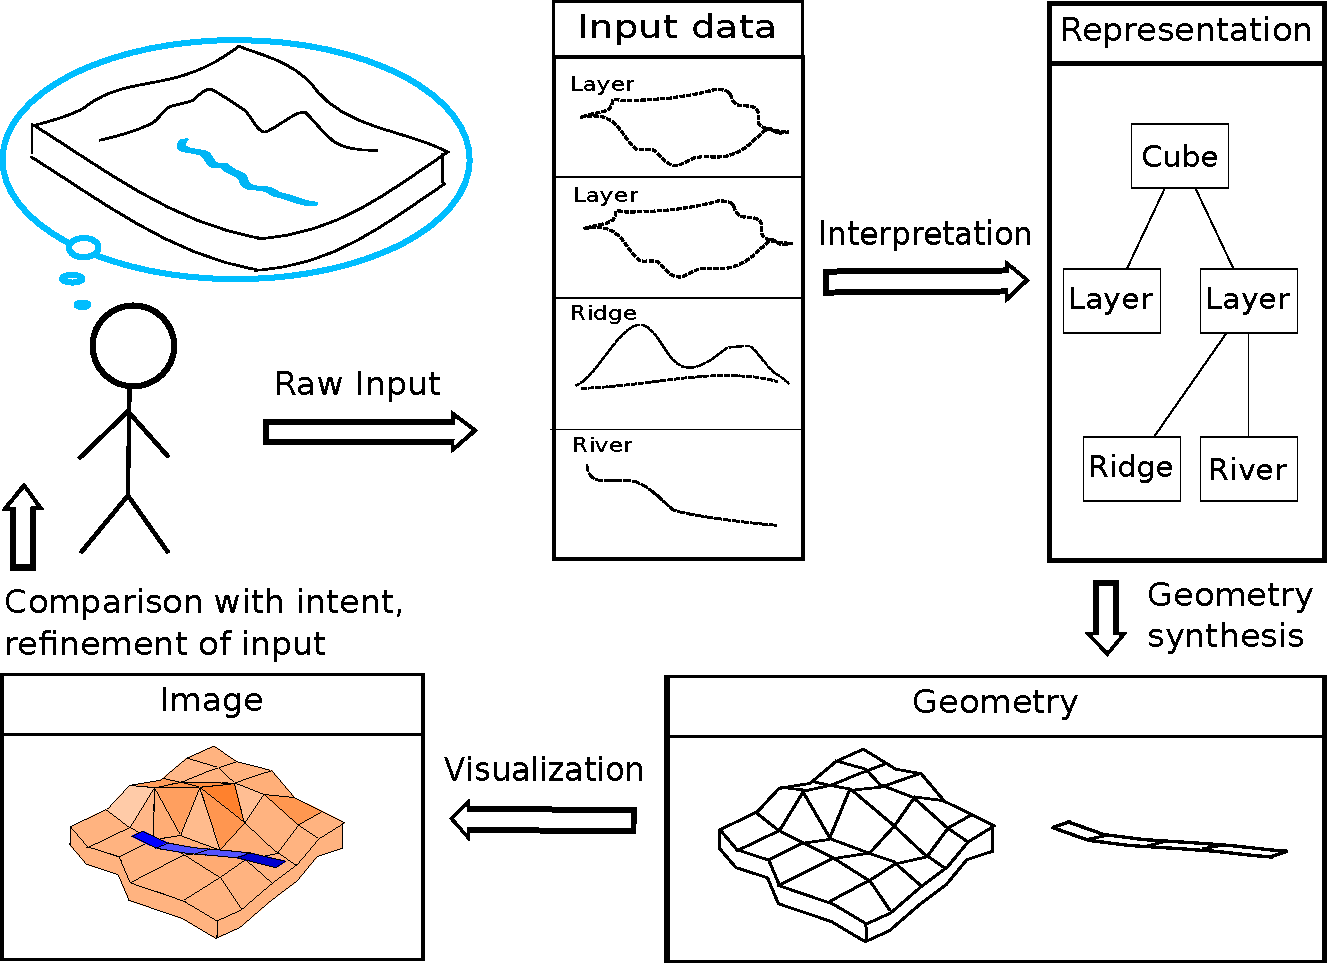
\includegraphics[width=\linewidth]{../thesis/overviewConcept.pdf}
 \caption{Conceptual overview.}
 \label{fig:overviewConcept}
\end{figure}

\begin{figure}
\centering
 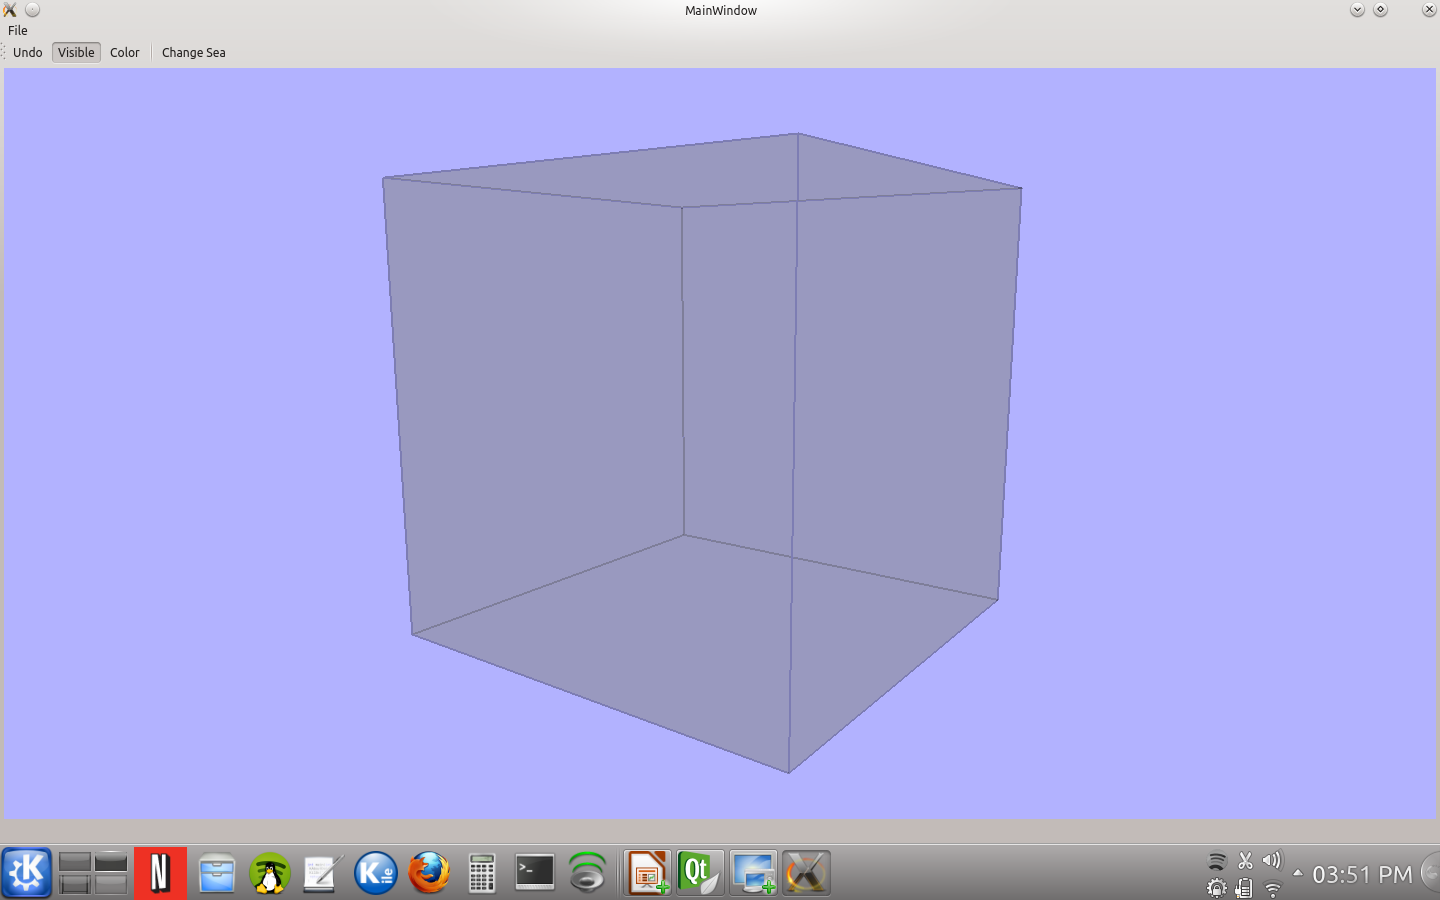
\includegraphics[trim = 50mm 30mm 50mm 30mm, clip,width=0.5\linewidth]{../thesis/emptyCube.png}
 \caption{The initial state is the empty cube.}
 \label{fig:emptyCube}
\end{figure}
The initial state for input is the empty cube (Figure \ref{fig:emptyCube}). At this stage the input consists of the user rotating the camera around the cube and drawing on the cube to create layers. The users input is projected from the screen space coordinates onto the geometrical model ( see Figure \ref{fig:intersect} ).There is a structure for each object in the scene that contains all the triangles that it consists of. Each of the vertices of the triangles are stored together with a two points that serve as the parameters that uniquely represent the point on the 2D manifold of the object. 

When drawing on a screen you are limited to the resolution of the screen. This means that the input points that are gathered will also be limited to this resolution However, because the actual surface where you are interested in drawing exists in a point in space farther away and not on screen, moving from one pixel to the next, means you will move a much greater distance on that surface than on screen, creating jaggedness. The input is smoothed by regarding the n points of the  input as the control points of a n-dimensional Bezier curve. The Bezier curve will approximate the control points, but will lie somewhere between them. Most of the points will lie on either side of the intended line, while a bezier curve will lie somewhere between.


 \begin{figure}
\centering
 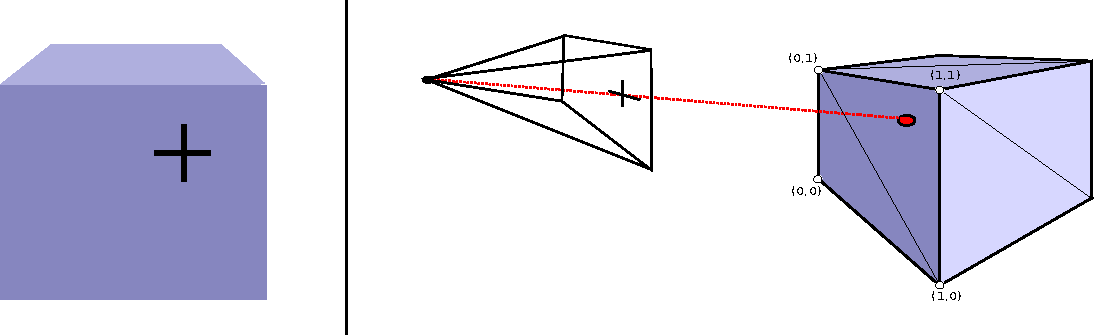
\includegraphics[width=\linewidth]{../thesis/intersection.pdf}
 \caption{Illustration of intersection. Left: the view of the user with a black cross representing the mouse cursor. Right: The point of the mouse cursor is projected onto the objects by creating a ray from the camera through the cursor and checking for intersections with objects in the scene. The numbers indicate the parametric space values of the vertices of the surface.}
 \label{fig:intersect}
\end{figure}

The different features that can be drawn are represented in an internal representation before creating the structure that can be visualized. The representation is also visualized to the user, so she can make changes.Most of the features that can be drawn are built by using the curves the user drew in different combinations and using different interpretations. In many cases the curves are augmented by some additional information, such as the height of ridges. With the deposits however, the representation does not include lines at all but the shape is rather defined by a procedural method.

All the features relate to each other in a child-parent relationship creating a tree structure. The cube is the top node in this tree. All layers are children of the cube. All the other features are then the children of a layer. This structure together with the parametric representation is useful to enable incremental refinement of features, meaning that any part of the whole structure can be modified at any time, without the user having to redraw every part that relates to that change.

Features have algorithms for creating geometry whenever the representation changes. These algorithms create triangles that are drawn on the screen by simple OpenGl functions. In order to achieve the transparency effect, features with geometry must be drawn in the correct order. Layers are drawn first, schetched curves second, rivers third, the sea fourth, and the cube last. This ensures that transparent objects are drawn last and from back to front. 

The cubes geometry is generated based on width, depth and height. It is created by six surfaces, representing the faces of the cube. The user sketches input for layers on the front, back, left, and right hand surfaces. A suggestion algorithm will add lines on the other faces, so that minimal input is needed if the user is satisfied with the suggestion. If further changes are made another algorithm makes sure the four curves are always aligning at the corner points, by modifying any previously drawn lines to align with the new one. The cube will also maintain a hidden set of curves that represent the top of all previously drawn layers. This eases the creation of new layers.

A layer gets these four sketched curves as input, plus the hidden curves. The top horizon of the layer is created by a custom interpolation algorithm ( see Figure \ref{fig:layerCreation}). 
The algorithm starts by doing a bilinear interpolation of the four corner values at the point of consideration. Then a linear interpolation of the two points of the front and back curves currently being considered. The difference between the points of these first two interpolations is then calculated. Another linear interpolation is done between the two points of the left and right curves at the point of consideration. To this last point the previous difference is added. The effect of this algorithm is analogous to the wooden profile explained earlier being dragged across the left and right curves while the actual wooden profile is being interpolated between the front and back curves. The result is the same no matter if viewed as if dragging the front and back interpolated curves across the left and right curve or vice versa.

Once the horizon surface is created, additional geometry is made at the side of the layer inbetween the top of all the previous layers and the new one. The Layers geometry need to update when child features are added or changed, and child features must update when the parent layer is changed. Because the child feature is always defined by the 2D point in the manifold of the parent, it is easy to make changes incrementally to layers.




\begin{figure}
 \label{fig:layerCreation}
 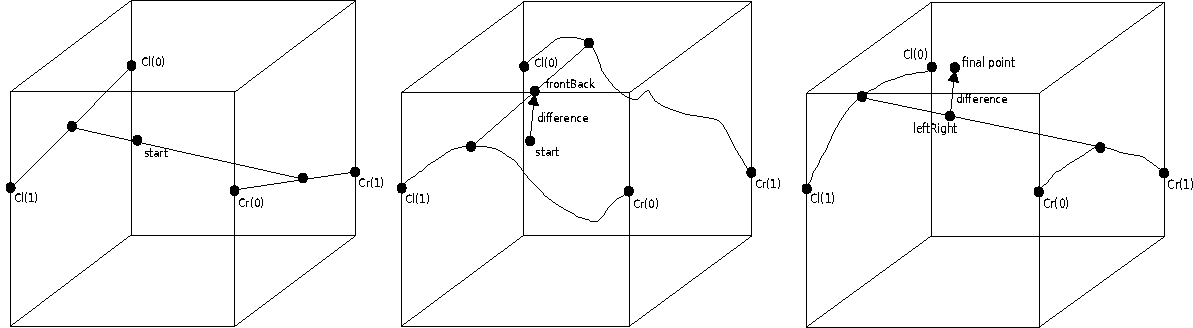
\includegraphics[width=\linewidth]{../thesis/layerCreation.pdf}
 \caption{The calculation of a point in the layer grid. First, find the starting point by interpolating the four corners for the current position in the grid. Second, interpolate the front and back curves at the current position, and calculate the difference from the starting point. Third, interpolate the left and right curve at the current position, and finally add the previously calculated difference to this point, yielding the final point.}
\end{figure}

Rivers can be drawn on top of the surfaces by indicating its path with a curve. An algorithm then creates a river as shown in Figure \ref{fig:riverDraw}. 
The input capture of the initial curve of the river is achieved by drawing on the surface as explained earlier.

The initial curve is interpreted as the center point of the river. Each of the two sides is then computed by extending a new point in both directions from the center point along the rivers path. At the ends of the river a logarithmic function is used to create a smooth falloff towards zero, to make the two sides meet. The initial line is discarded. The two sides of the river become the representation of the river, and they are the lines that can now be further modified by the user by oversketching. 

The oversketching is done on one side of the river at a time. The user also has the choice of replacing the entire side of the river if that will let her more easily make the changes she wants.
When oversketching or changing the sides of the river, the layer geometry as it was before the river made any changes is used for the intersection tests. This is because it gets difficult to draw a new side of the river outline on the surface, if that side goes inside the river itself, as the terrain in that area is deformed by the river.

\begin{figure}
\centering
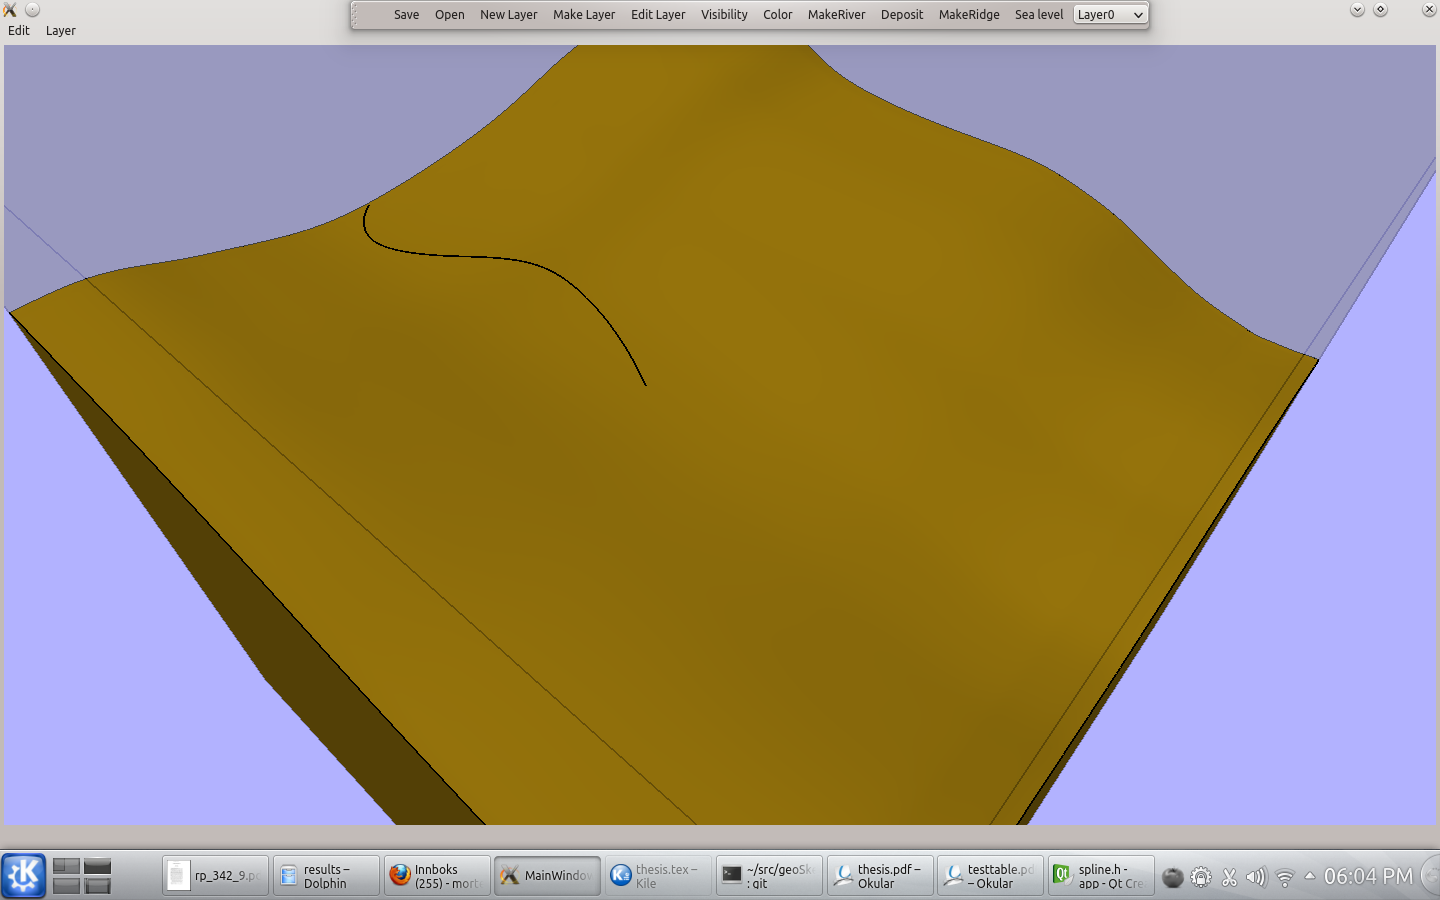
\includegraphics[trim = 30mm 80mm 120mm 30mm, clip,width=.4\linewidth]{../thesis/results/riverDraw.png}
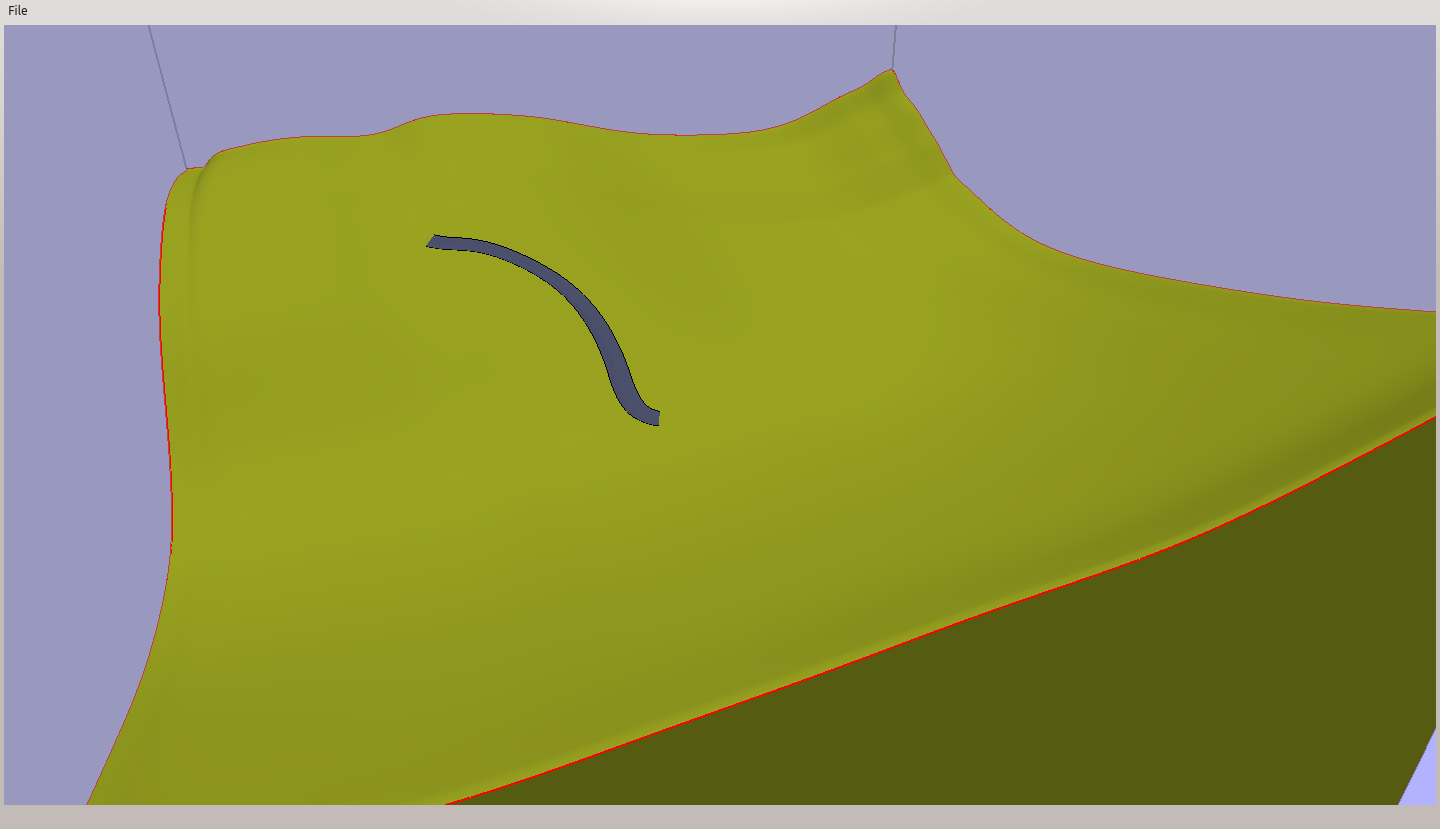
\includegraphics[trim = 30mm 80mm 120mm 30mm, clip,width=.4\linewidth]{../thesis/results/riverDrawn.png}
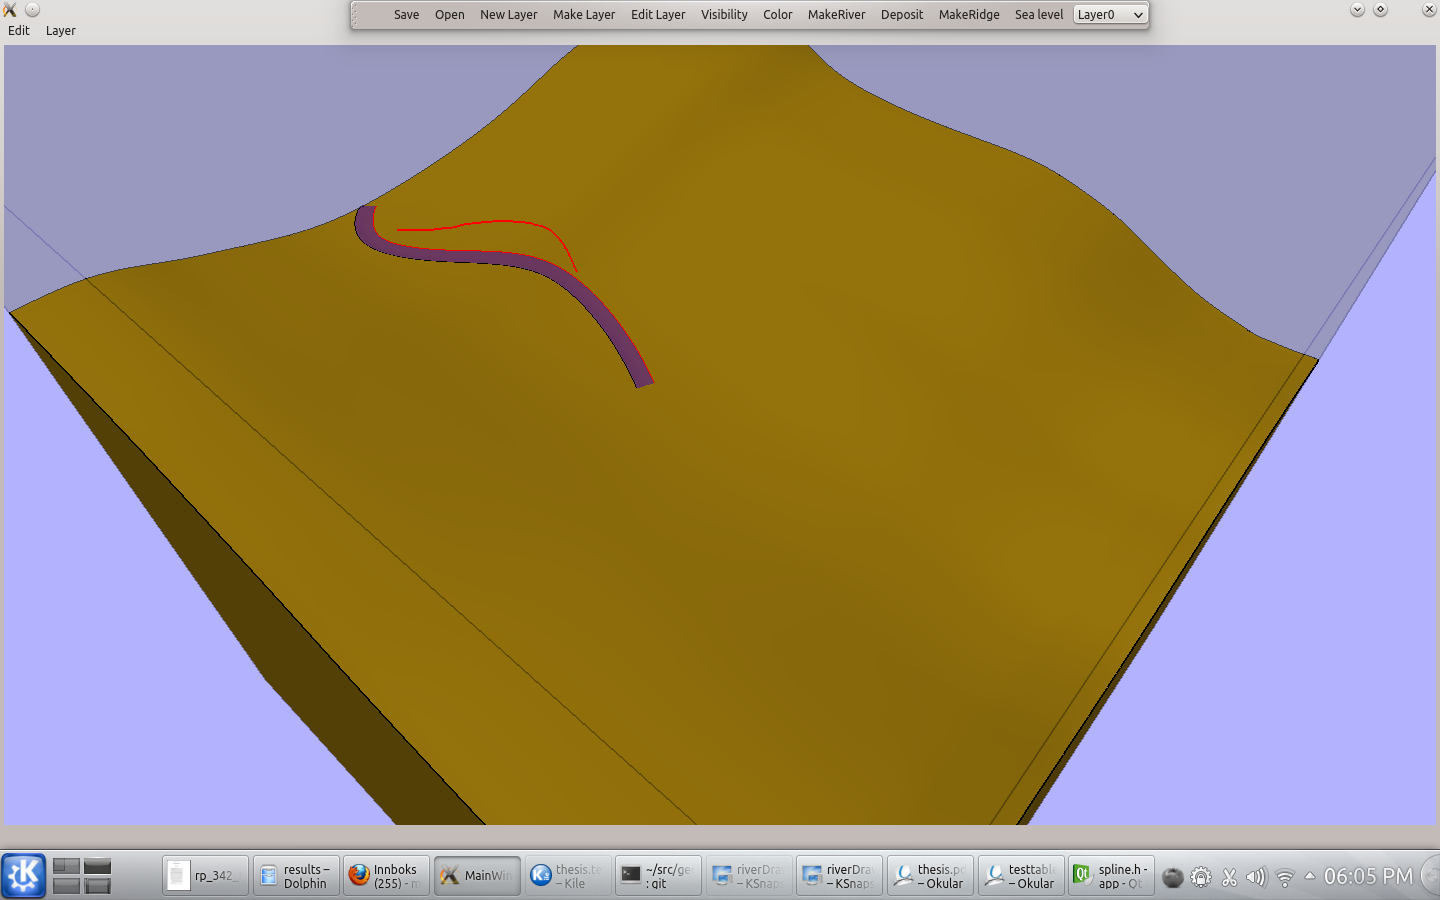
\includegraphics[trim = 30mm 80mm 120mm 30mm, clip,width=.4\linewidth]{../thesis/results/riverChange.png}
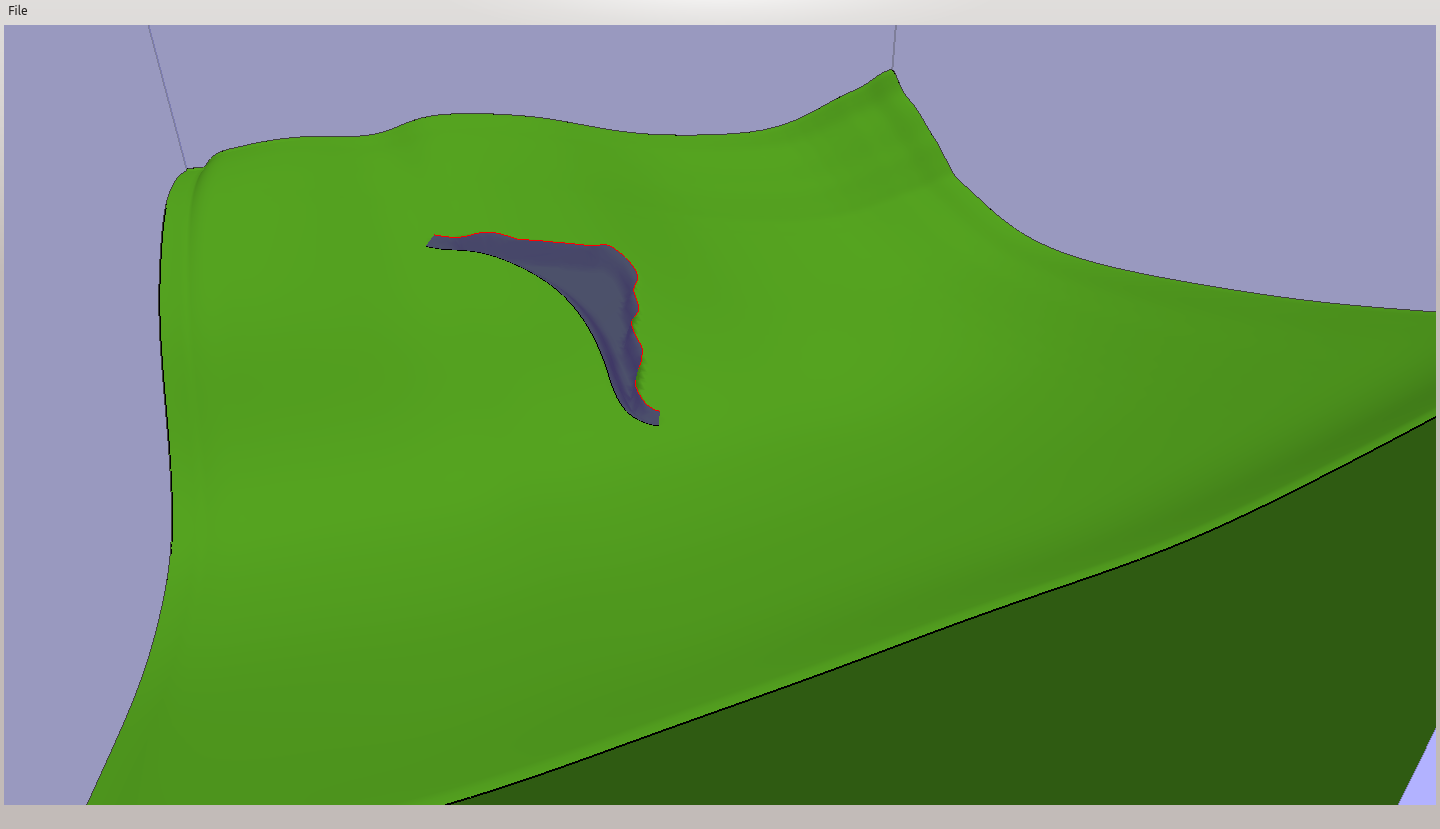
\includegraphics[trim = 30mm 80mm 120mm 30mm, clip,width=.4\linewidth]{../thesis/results/riverChanged.png}
 \caption{Sketching of rivers by indicating where it should run (top), and oversketching of the sides (bottom). }
 \label{fig:riverDraw}
\end{figure}
A valley functions almost identical to a river, only it does not create a geometry for any water and is initially wider and deeper than the river. It is, like the river, made by first drawing a line and then it can be changed by the same mechanism as the river. I will therefore not go into more details about the valleys.


Ridges are also drawn by a line on the layer surface. Once a line has been drawn and the user indicates that she wants a ridge, a generic shape of a ridge is created automatically as seen in Figure \ref{fig:ridgeDraw}. The user then has the choice to change the height profile along the ridge's baseline. This is done by sketching on a temporary sketching surface that is constructed along the ridges baseline.

\begin{figure}
\centering
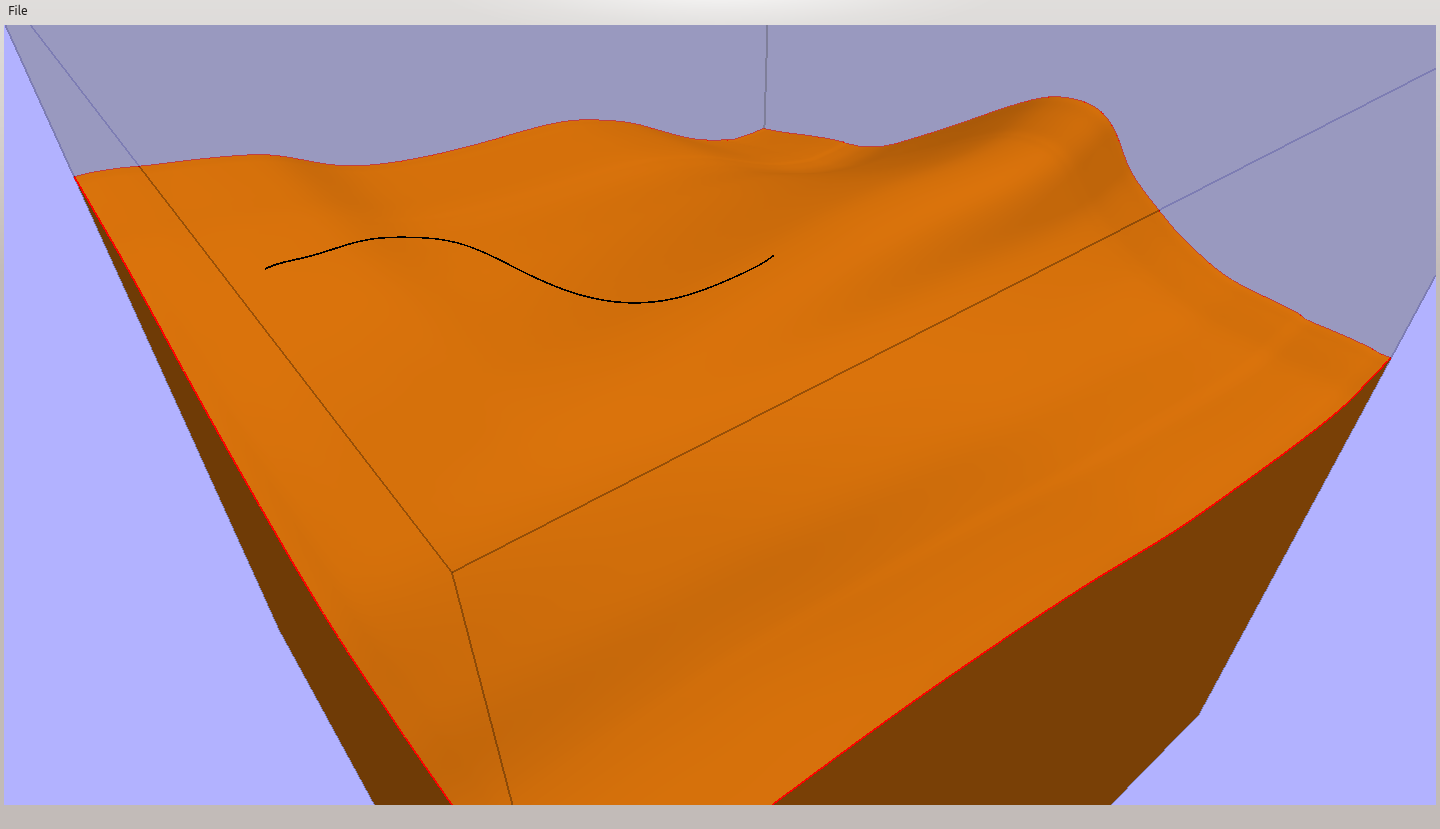
\includegraphics[trim = 30mm 80mm 120mm 30mm, clip,width=.4\linewidth]{../thesis/results/ridgeDraw.png}
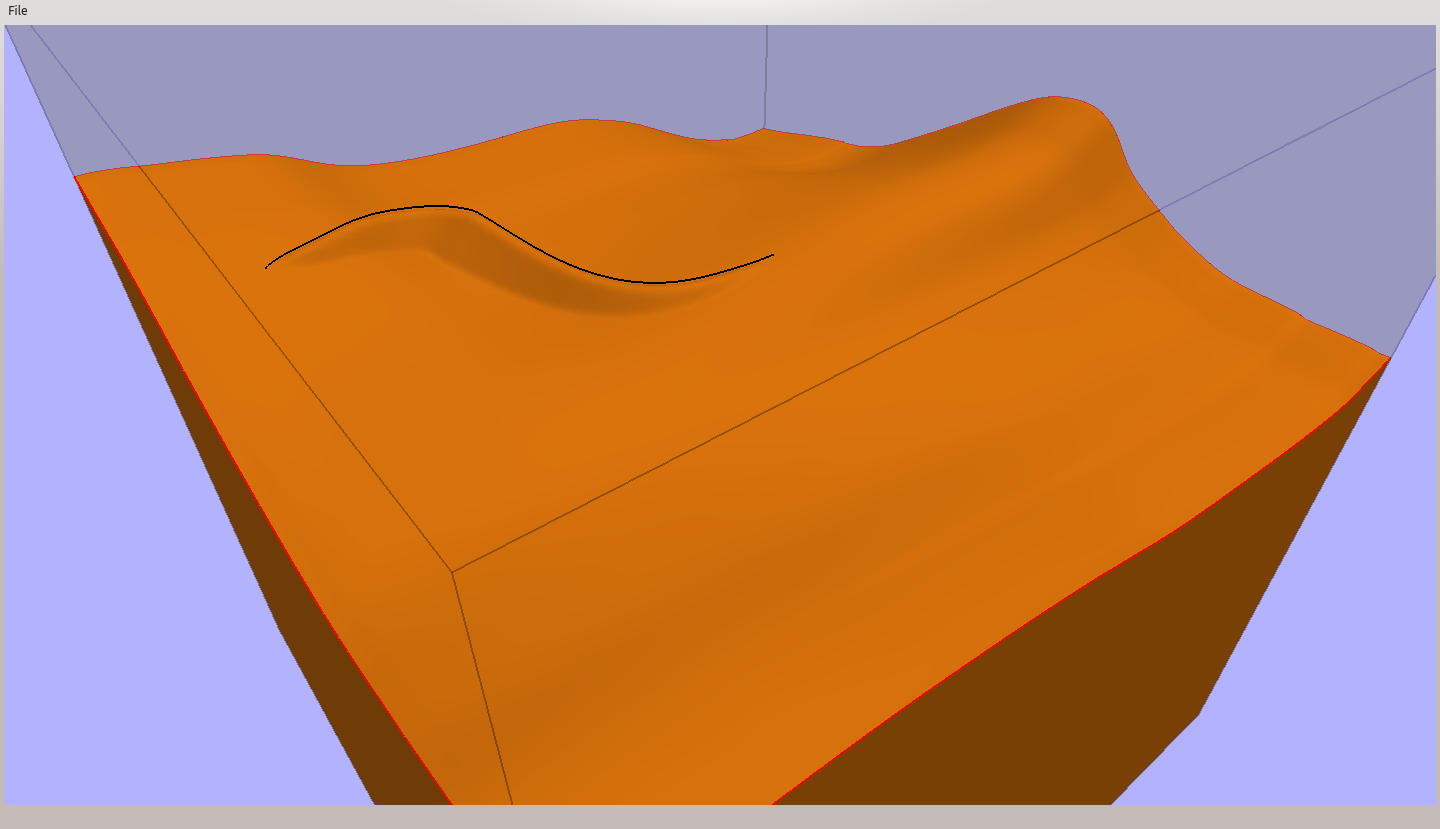
\includegraphics[trim = 30mm 80mm 120mm 30mm, clip,width=.4\linewidth]{../thesis/results/ridgeDrawn.png}
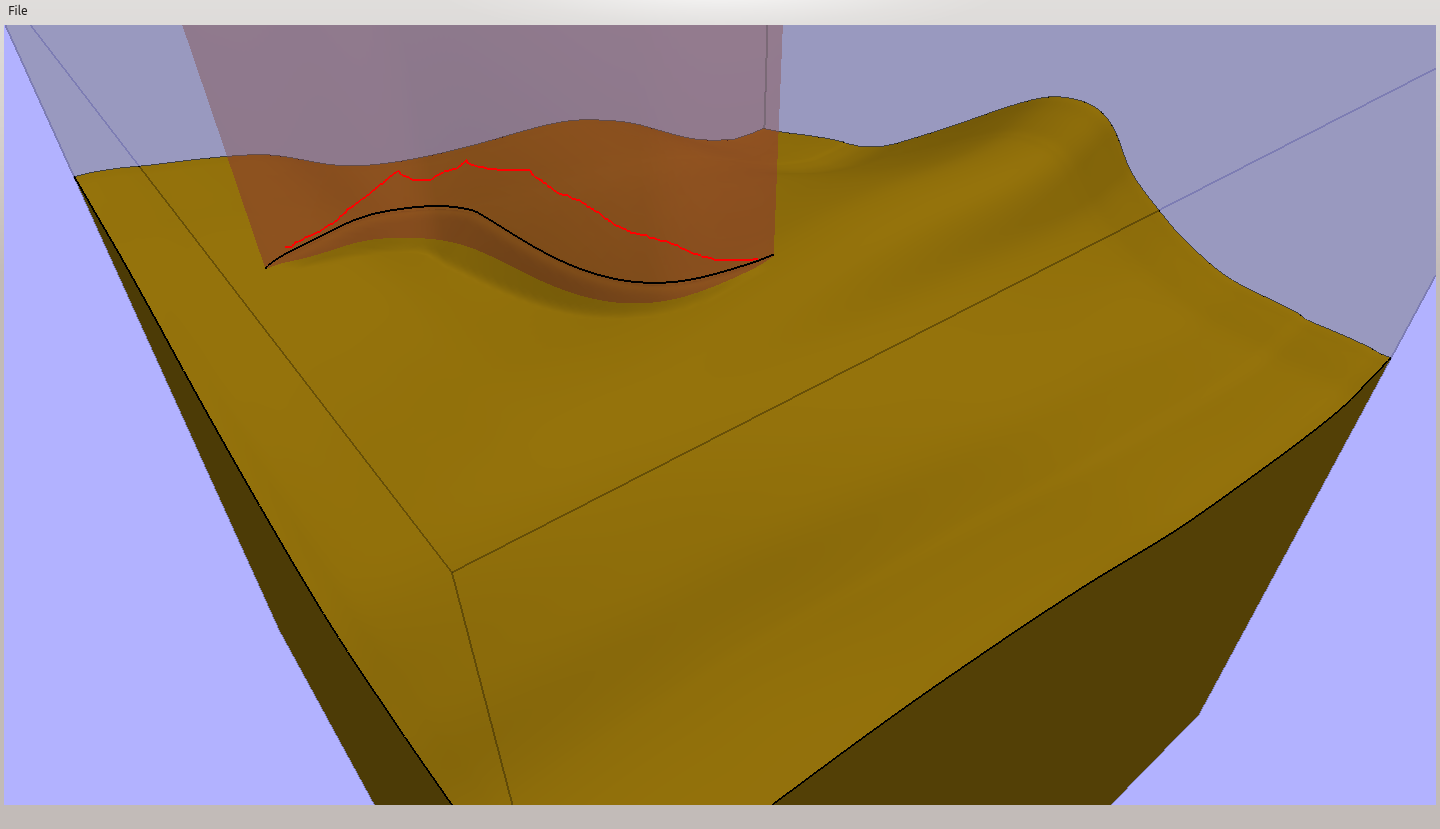
\includegraphics[trim = 30mm 80mm 120mm 30mm, clip,width=.4\linewidth]{../thesis/results/ridgeChange.png}
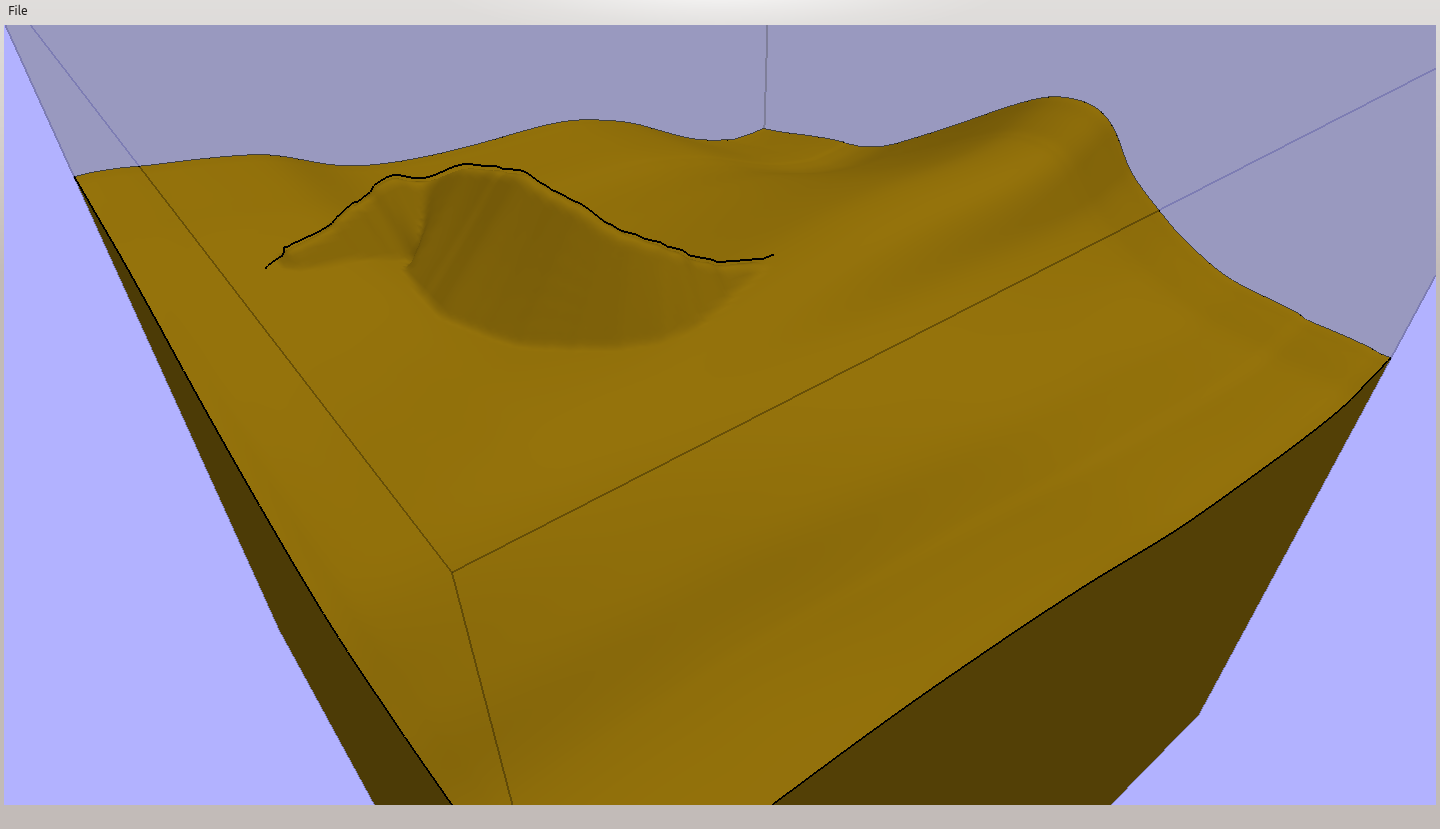
\includegraphics[trim = 30mm 80mm 120mm 30mm, clip,width=.4\linewidth]{../thesis/results/ridgeChanged.png}
 \caption{Sketching of a ridge by indicating where its base goes (top), and changing it by sketching the height (bottom). }
 \label{fig:ridgeDraw}
\end{figure}

Input for the ridges is first drawn on a layer as a curve. A ridge is represented by this curve and a height associated with each point in the curve. The curve is the base line that the user drew on the layer where she wants the ridge to follow along. The heights are the height of the ridge at each point of the curve. Initially the height list is just a smooth function from side to side of the ridge, with a peak in the middle. The height can be changed if the user indicates so. This new height line is input on a temporary sketch wall constructed for this purpose. The input procedure is similar to other lines, but in the end it is not actually stored as regular curve. When the user is done inputing the height line, the height along the entire wall is stored in a list, one for each point on the base line.

The ridge object itself is visualized only by a contour along the top of the ridge. This is constructed by iterating along the points of the base line. For each point in the base line, the corresponding 3D point is found by looking up this point on the layer the ridge belongs to, that is its parent. Afterwards, the height of this point is simply increased based on the relevant height in the list. This yields a new list of points which can then be used to draw a line on screen. When the height of the ridge is being changed, the sketch wall is also shown. The sketch wall is transparent to let the user see other structures that lie behind, so that it is easier to judge how high to sketch.

The sea level can be enabled at any time and moved up or down as the user specifies. The sea level is implemented simply by creating a layer with straight outline curves. Each time any layer changes the sea level layer is recomputed. The input is made on the cube by clicking the mouse after having indicated by a button that one wishes to change the sea level. It is visualized with a transparent blue color. In addition to being used in scenes to illustrate the sea, the sea level is used as an input parameter for creating deposits. 

Sedimentary depositions can thus be modeled where a river meets the sea. The user indicates which river is to start depositing, and the rest is done procedurally by a simple simulation. The procedure continues until the user stops it. The user can indicate more than one deposit to be made for a single river. This will make the deposits build outward on top of each other in the direction of the river while also following the terrain.

In order to visualize the creation of a deposit as it builds over time, it needs an additional step to generate an intermediate representation of the deposit before generating the geometry. This step consists of simulating the flow of matter across the surface underneath. For the simulation a simple volume preserving diffusion algorithm is used, that is a modified version of the one by Boeschs \cite{Boesch:2011:Online}. An illustration of the approach by Boesch is given in \ref{fig:boesch}. The algorithm works by considering one cell at a time, and comparing the heights of the neighboring cells height from the previous iteration. Half of the difference, clamped by the available amount of water, will be added to the current cell. This is first done for each cell considering its neighbors along the x-axis. Then the process is repeated, but this time considering the cells neighbors along the y-axis.  In my version of the algorithm, even less than half of the difference is added according to how far from the 
rivers mouth the cell is.  This algorithm assumes a regular height grid, and all the underlying layers must be taken into account. The layers are represented as a irregular grid and thus a sampling must be performed to create a regular grid. At regular intervals, a ray is cast directly down into the cube, doing intersection tests for each layer, updating a value in a regular height grid to the height of any intersection when that intersection is higher than the 
current value. After the grid heights are found the simulation begins.
\begin{figure}
 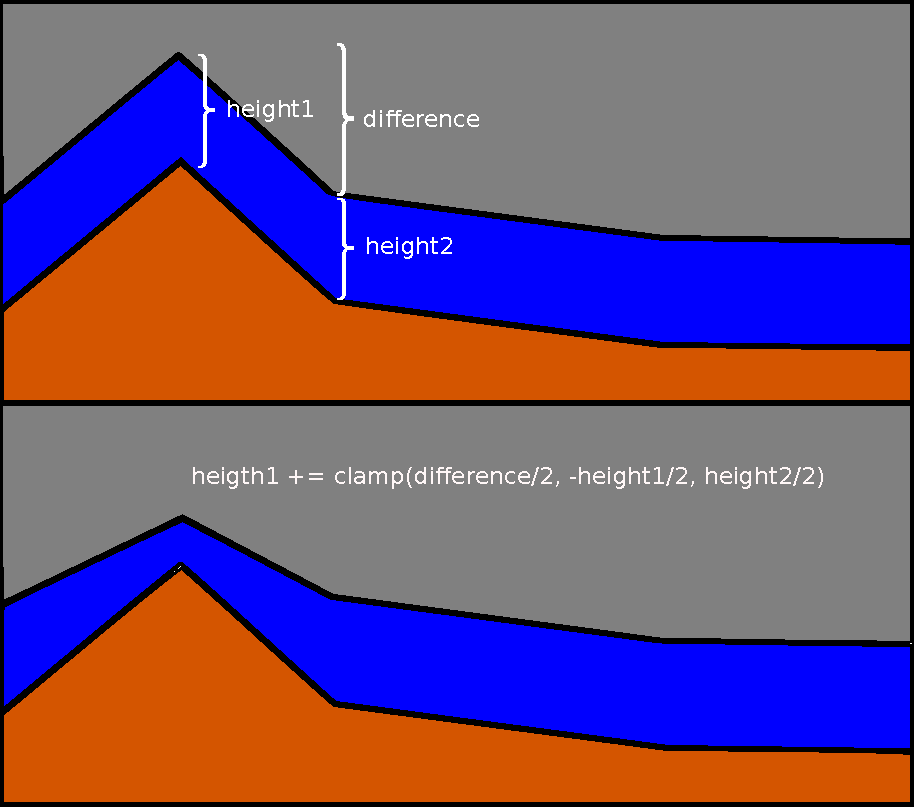
\includegraphics[width=\linewidth]{../thesis/diffuse.pdf}
 \caption{Recreation of figure from approach by Boesch \cite{Boesch:2011:Online}.}
 \label{fig:boesch}
\end{figure}

The simulation runs until the user is satisfied and stops it or if the deposit is a preexisting one, until the target deposit amount has been reached. The total amount of deposited matter is stored in the target variable when the user stops the simulation. Geometry is generated based on the height of the deposits and underlying terrain. When generating geometry special care needs to be given to the orientation of the triangles to give a uniform and smooth look to the visualization.

To decide where to add triangles, and in which orientation, for the space in between each of the grid cells, the four surrounding points are considered. If both the lower right and upper left cell has deposited material, then triangles will be created between these two cells and one triangle for the two other cells if they have material deposited to. Otherwise, if both the upper right and lower left cell has material deposited, then triangles are created using these two points and creating one triangle extending to each of the other two points as illustrated in Figure \ref{fig:triangleOrient}.

\begin{figure}
 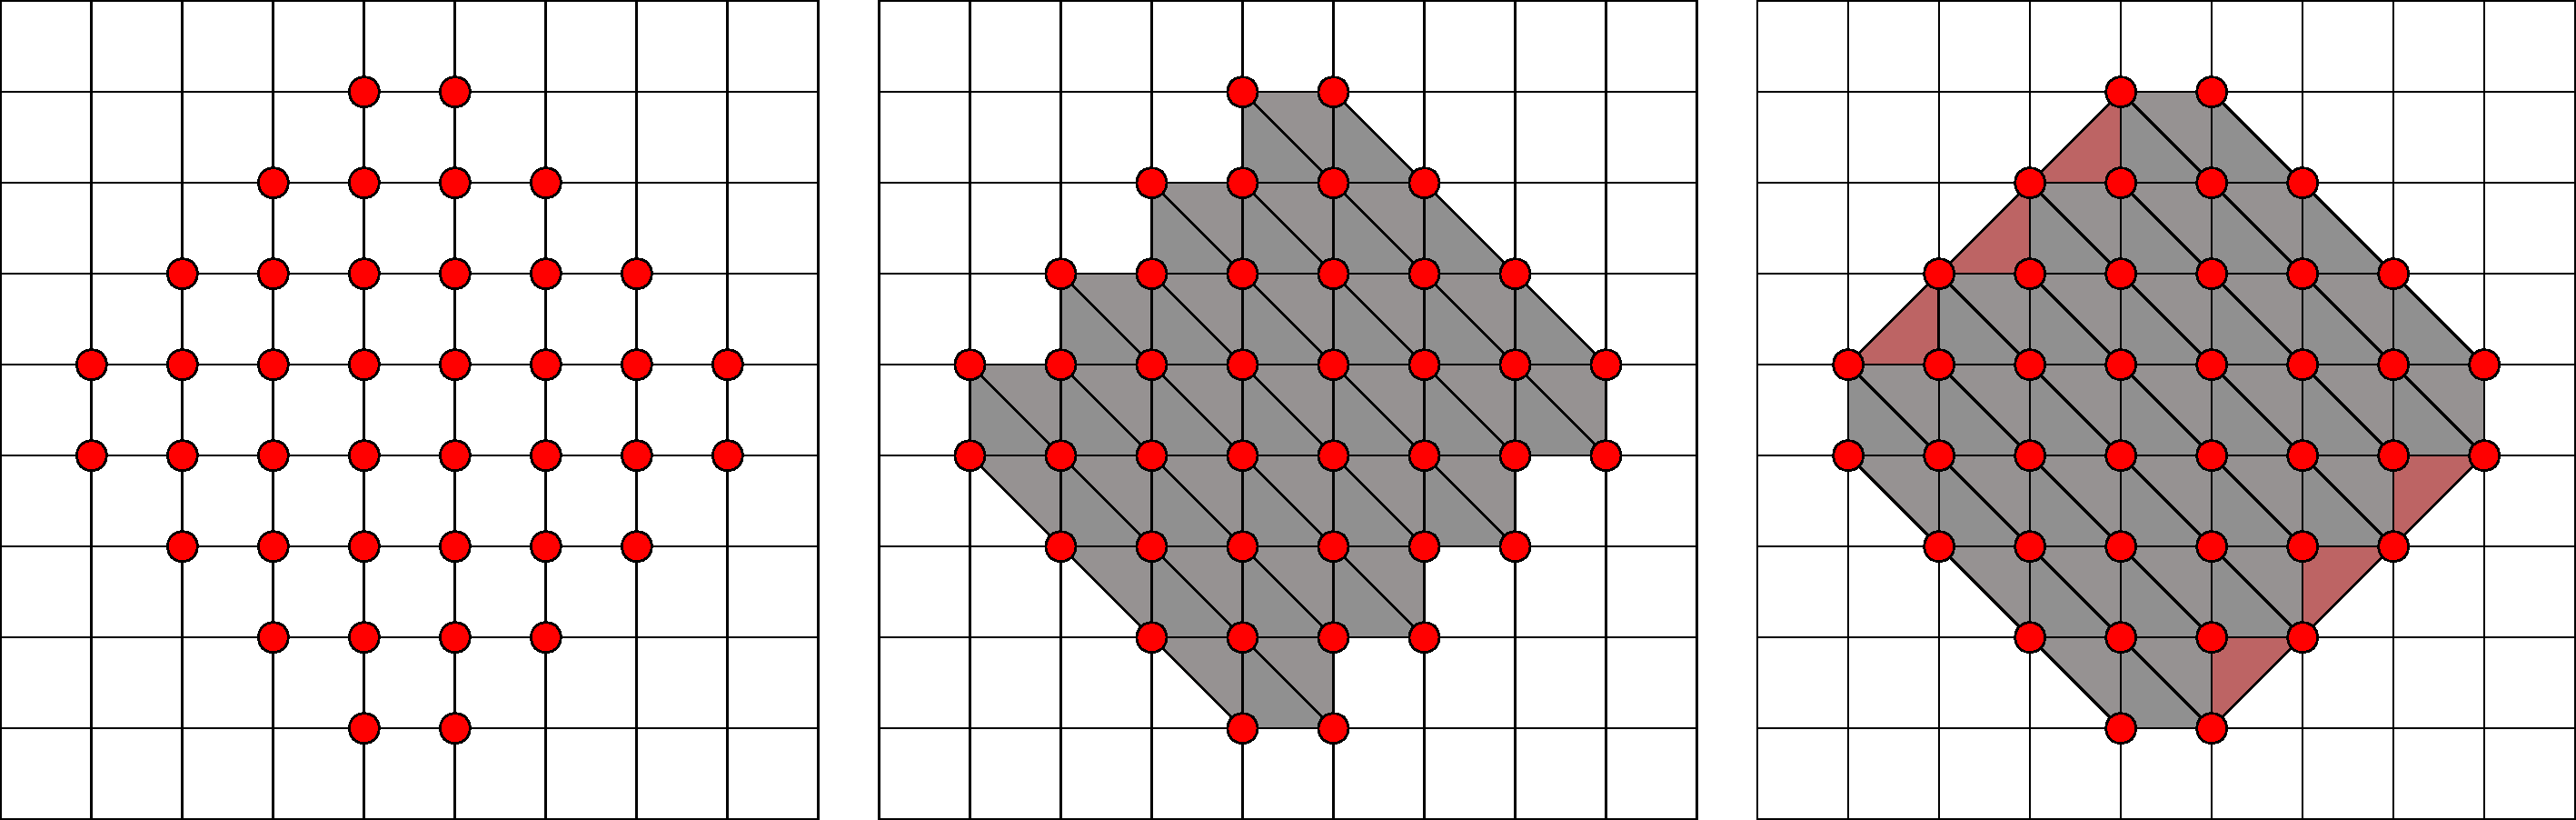
\includegraphics[width=\linewidth]{../thesis/gridtrianglesall.pdf}
 \caption{Triangle orientation. Left; the grid points that have matter deposits above the threshold. Middle; the first, naíve approach where all triangles are oriented the same direction. Right; the more sophisticated approach, where the triangle orientation depends on which surrounding points have deposited matter. As seen on this illustration, the second approach gives a more uniform look on each side of the structure, while the first approach gives more jagged edges and non-uniform look.}
 \label{fig:triangleOrient}
\end{figure}

When creating a deposit, the layer object will check for previous deposits, and if such exists, the grid data will be reused for the next deposit. It is reused by copying the terrain height grid and then adding the height of deposits at the points of the grid. This gives speed improvement, and also enables deposits to stack on top of each other.

\section{Results}
Figure \ref{fig:sketchRepro2} shows the same scene as reproduced by the author of the program along with a ray-traced image made in the program Blender. This sketch is made by drawing two layers and setting a color for them. Then some mountain ridges are added. A valley is created between the ridges, and in it a rivers path is sketched. After the sea level has been indicated, some deposits are created at the point where the river meets the sea.

\begin{figure}
\centering
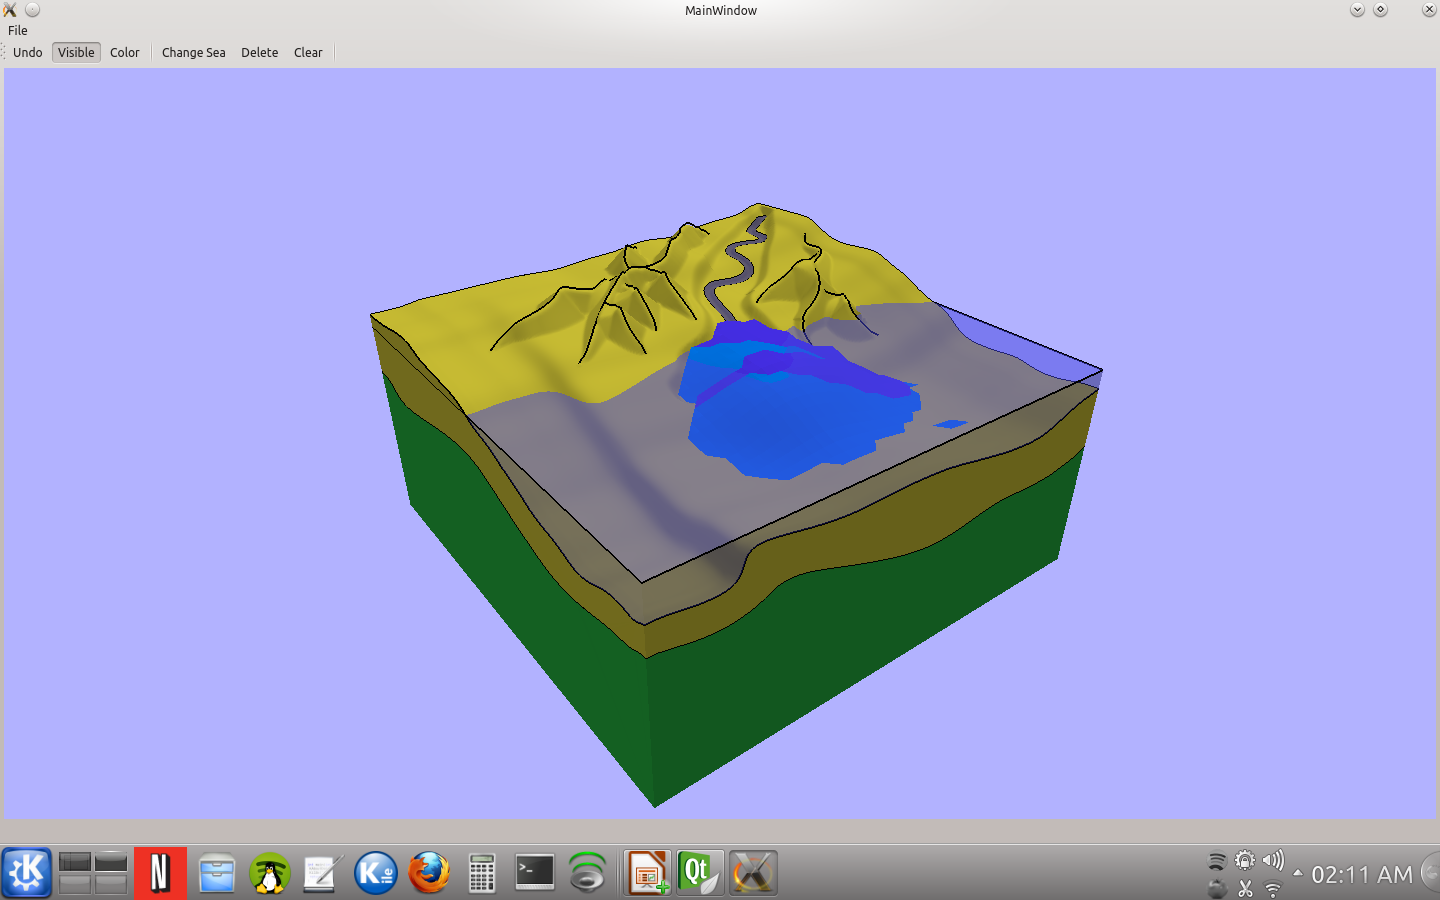
\includegraphics[trim = 90mm 22mm 80mm 30mm, clip,width=.4\linewidth]{../thesis/resultsSection/sketch/author.png}
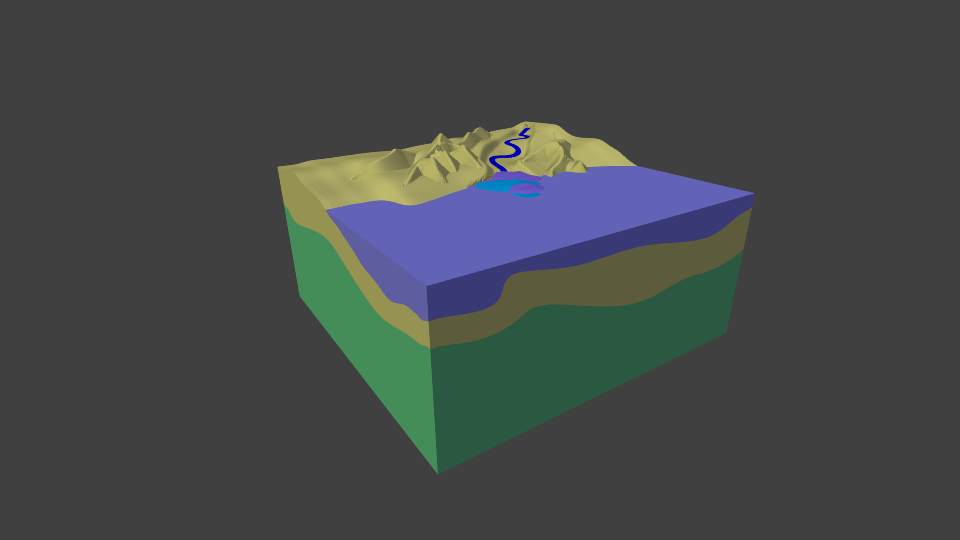
\includegraphics[trim = 40mm 0mm 30mm 9mm, clip,width=.4\linewidth]{../thesis/resultsSection/sketch/authorBlend.png}
 \caption{Imaginary terrain sketched, and a rendering made by ray-tracing the exported geometry.}
 \label{fig:sketchRepro2}
\end{figure}

Figure \ref{fig:glacier} shows the process of how a glacier erodes the landscape. The first sketch is made by drawing the outline of the rock with valley from the first illustration, then simply adding some ridges and rivers. The second sketch is then made by editing the layer to create the valley that is carved by the glacier and deleting the rivers. Then the glacier is created by drawing the end lines on the front and back of the glacier as the contours of a new layer. On the other two sides, the slope of the glacier is indicated. The third sketch is then made by deleting the glacier layer, adding some new rivers and valleys, setting the sea level, and creating a small deposit. 

\begin{figure}
\centering
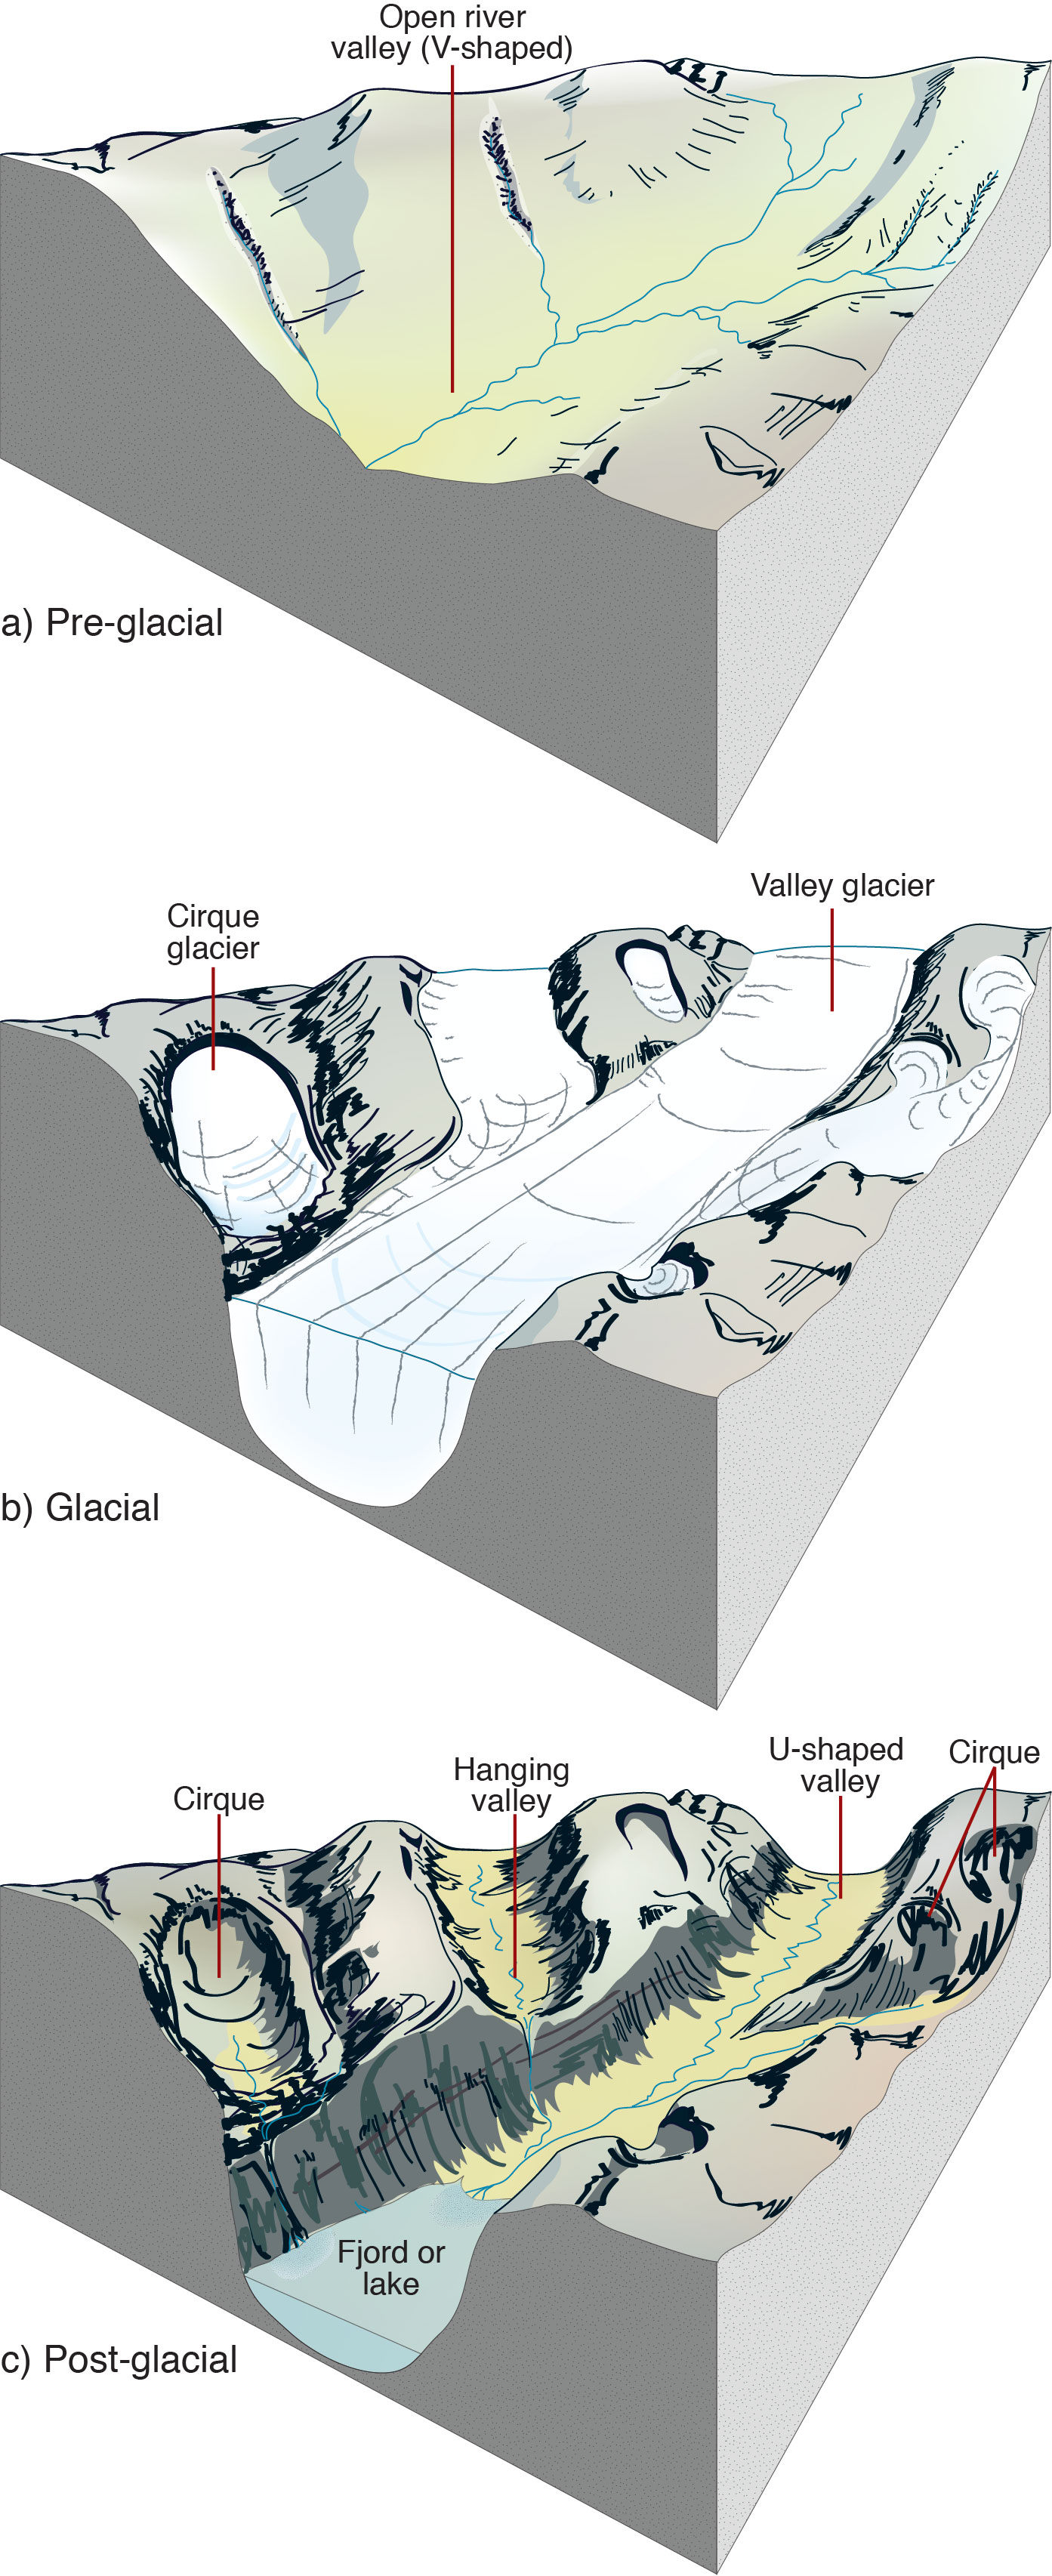
\includegraphics[width=.4\linewidth]{../thesis/geo/english/ice.jpg}
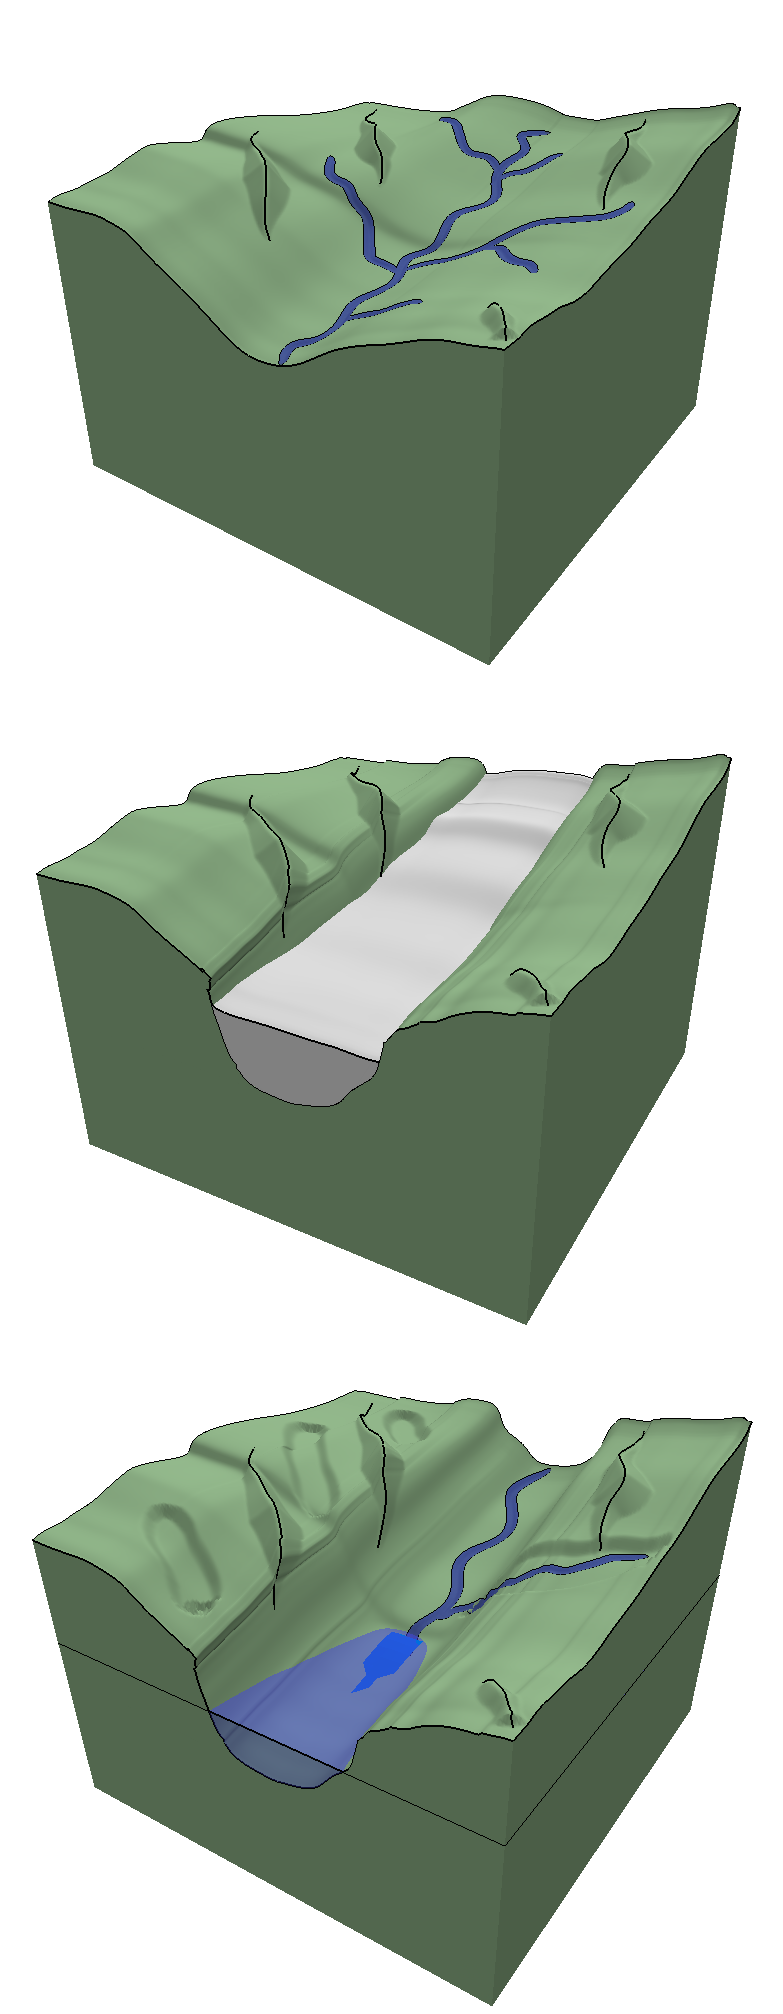
\includegraphics[width=.4\linewidth]{../thesis/resultsSection/iceSketchTriple.png}

 \caption{Glacier illustration and attempt at reproduction.}
 \label{fig:glacier}
\end{figure}

Figure \ref{fig:subduction} shows the process of how the oceanic part of a plate is submerged underneath a continent on another plate where they collide. The structures have to be build from bottom to top, or rather any layer that intersects another must be drawn last. The mantle must be drawn even though it does not appear in the sketch. It is shown in gray here for illustration, but it could be made invisible. Then the oceanic lithosphere is drawn, the oceanic crust follows. Then the continental lithosphere and the continental crust is drawn such that the sketched curves intersect the oceanic crust at the subduction point. The last layer is the accretionary prism, which represents sediments scraped of from the subducting oceanic plate and gathered at the wedge between the plates. Finally, the sea level is indicated, some ridges of mountains are added and an inland sea is created by drawing a river and widening it. The melting rock, rising magma and other volcanic features can not be recreated at this point.
\begin{figure}
\centering
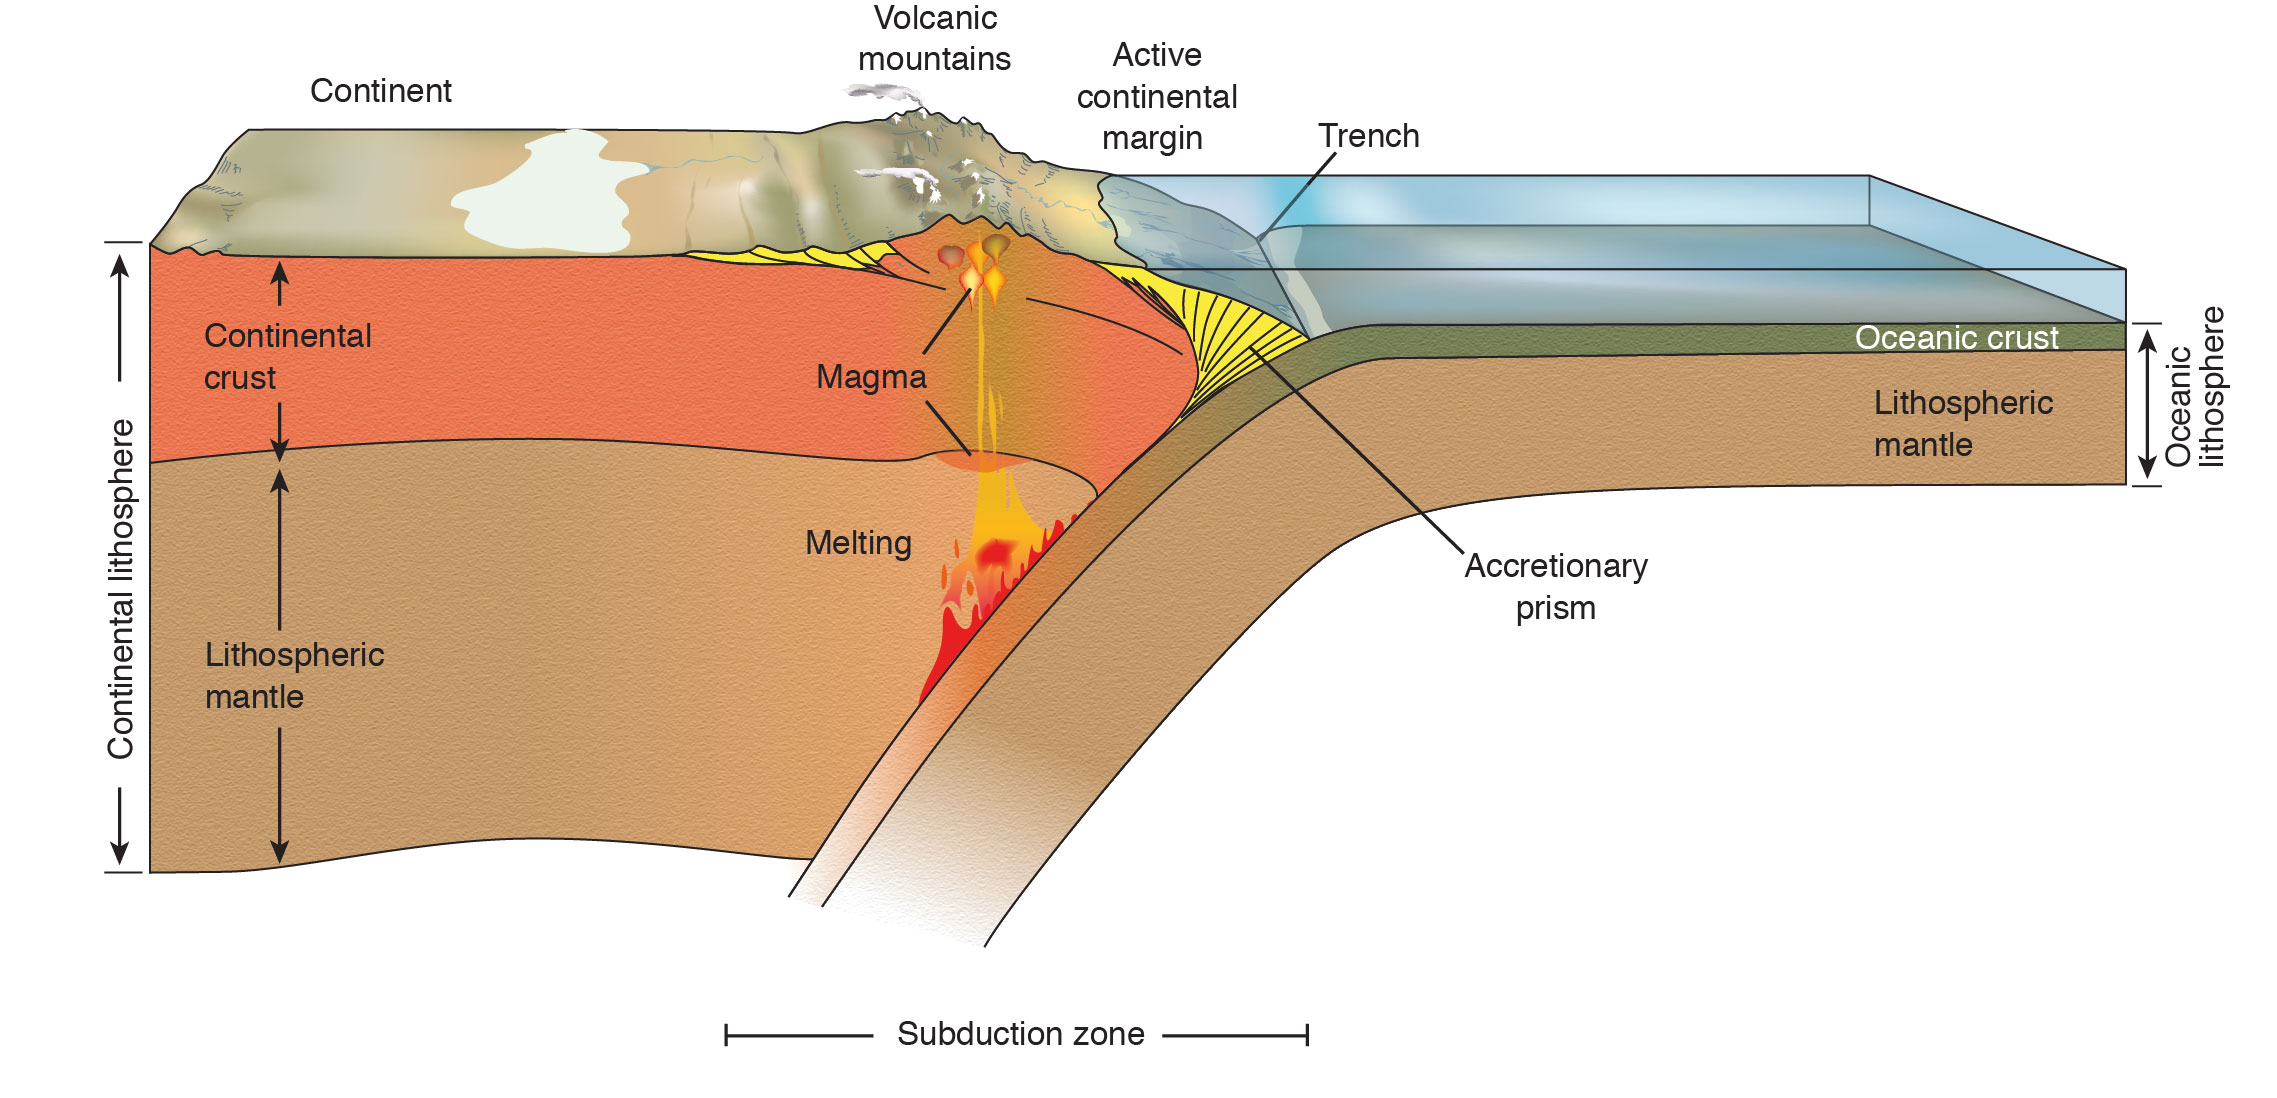
\includegraphics[width=.5\linewidth]{../thesis/geo/english/subductionCont.jpg}
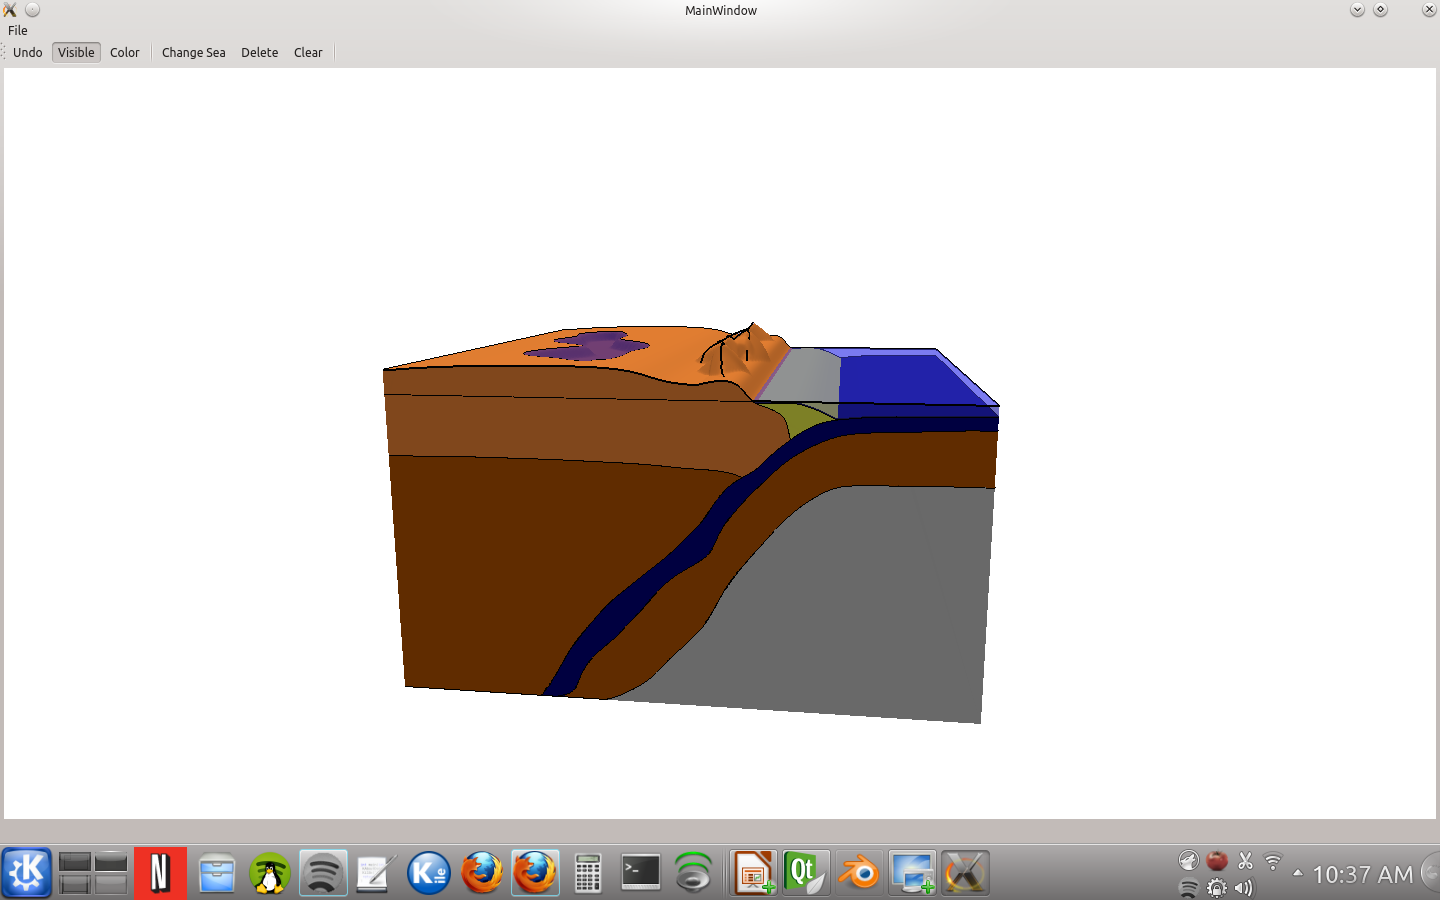
\includegraphics[trim = 50mm 30mm 50mm 50mm, clip,width=.49\linewidth]{../thesis/resultsSection/subductionSketch.png}

 \caption{Illustration of subduction of oceanic lithosphere underneath continental lithosphere and attempt at reproduction.}
 \label{fig:subduction}
\end{figure}


\section{User study}
Evaluating the usability of a modeling approach is not easy. The study was conducted to gather feedback from a group of geology students. The study consisted of several questions relating to the different aspects and features of the approach. The answers had to be given by indicating on a scale from 1 (worst) to 10 (best) according to how much the user agreed to a question, liked or disliked a feature, etc. In addition the subjects were given the opportunity to explain their choices and give comments for each question. A summary of what the subjects responded is given here.

The subjects found the tool useful for making illustrations and found the look pleasing. However, the menu items were confusing for some. The ease of use was praised as the most significant advantage of the approach. The approach was described to give the ability to play with the different ideas and thoughts around geological scenarios. One user said he had never seen an approach giving the possibility to create simple illustrations as quickly and easily as this. The approach was described as very self-explanatory, and in particular one user was impressed with the ability to make changes to the illustration after having made a basic version of the scene.

Some users thought the approach was very easy to use, while others needed some more effort to learn it. There was also a suggestion to make a list for selecting the different objects in the scene, as that could sometimes pose difficulties. Some said that the tool can in its current form be useful for illustrating some very simple geological scenes, but that it would require more development for it to be useful for depicting more complex scenes. Suggestions for improvements was a feature for creating faults, the ability to alter the width of mountains and the depth of valleys.

One subject indicated a belief that if the features suggested could be implemented, the program could become very useful for them. Another said that the way they make illustrations today is usually by hand, which is very time consuming. This approach helps creating quick illustrations. One user remarked that it was very easy to make changes to layers, and that the methods of changing all the terrain features and rivers was excellent. This user also said it was important to not complicate this too much, since the strength of the approach lies in its simplicity.

\section{Further work}
I would really like to develop an intuitive approach for making fault structures in the layers. By my own understanding of geologist's needs, how often faults are encountered and based on test subjects feedback, fault structures would be the natural next step for further research. I think an easy way to input such faults could be to let the user sketch curves on each horizon where the intersection of faults and layers should be. An interpolation of these curves would then create a surface representing the fault. The user could then indicate by sketching on this surface how far the layers involved have faulted. Finally an algorithm would be needed that could morph the layers and any features already drawn on them.

Another feature I would like to see, is the ability to combine several cubes into a bigger scene. This would require some means of using what has already been sketched on one cube as a starting point for adjacent cubes. In order to not impose too much work on the user, the surface creation algorithm would need modification to ensure continuity of surfaces across cubes. I think that conducting further research into using the Inverse Distance Weighing interpolation approach, could help with this since it could take into account the points on both adjacent cubes in the weighting. The Discrete Smooth Interpolation developed by Mallet \cite{mallet1992gocad} would also be interesting to explore for allowing smooth transition between the cubes. The ability to change a cubes height, width and depth is another possible feature that could be useful. To make this cube change work together with the multiple cubes all cubes could be restricted to the same size, so they will align properly.

There is also a number of possible improvements on the features that are already included. The river width control can today be a bit difficult to use if the user wants to create narrow rivers. This difficulty could perhaps be removed if there was a way to change the width across the entire river in one go, instead of having to carefully sketch along the entire rivers length. Ridges could benefit from some method of sketching the width along the length of the ridge. I think both depth and width control could be achieved by additional sketching surfaces. If the user could sketch the profile in of a river, valley or ridge orthogonal to the direction of the initially sketched base line, I think this would be sufficient to create many desirable versions of such features. To make this feature even more powerful, it could be possible to input several such profiles along the length of the feature, and the profile could be interpolated between them.

To make deposits a more powerful feature, I would make them into fully fledged layers. By this I mean that it should be possible to modify them in all the same ways as the sketched layers in the cube. The procedure that creates the deposits could also have more parameters, like how far it will flow, how much material is transported, how fast the river flows, etc. It could take into account the possibility of the river stream carrying different sized particles at the same time, thus depositing them in different regions. The flow speed of the river could be calculated based on the terrain slope. The amount of deposited material would be dependent on several factors possibly outside the sketch, such as terrain material and length of river. Deposits could also benefit from more control over the shape.

Many of the illustrations could benefit from a feature that allowed painting on the surfaces of the sketch like Natali et al. \cite{natalirapid}, and by creating billboards such as Cohen \cite{cohen2000harold} suggests. Painting on the surfaces would for example allow the illustration of subduction of oceanic plates sketch in Figure \ref{fig:subduction} to be completely reproduced. A billboard feature would also allow geologist to input context giving features such as vegetation and animal life, plumes of smoke from volcanoes, etc. I would also like to see a texturing feature similar to what Natali et al. proposes where textures by default follow the layer structure, but the user can sketch to override its direction and deformation to illustrate details of a layers internal structure. Another way 
to add a more realistic look for the horizon surfaces could be through a fractal noise method.

If implementing any of these features it is important to focus on the usability and ease of use. In that respect I would continue to involve users from the geologic field. One of the characteristics test users have commented was the ease of use of the features and of creating sketches in this approach. If it would become more difficult to use, they might prefer to draw illustrations by hand. It should preferably not become more complicated to model the scenes that are already possible to create. New features should simply add possibilities that are as easy to use as the rest.

\section{Conclusion}

This paper started by explaining how geologists have a use for an application that lets them create simple models that lets them illustrate their thoughts amongst themselves. In education and literature such illustrative tools are also useful. A goal was stated: to create an approach for rapid and easy sketching of geologic structures in 3D. An approach for a tool for rapid modeling of geologic structures was given and how it was developed was explained in detail. The approach explained is mostly based on sketch input, but also incorporated a procedural method to explore the possibility of combination of these two rapid modeling metaphors.

Screenshots of geologic scenes that can be modeled using the currently implemented algorithms were given. A user study showed that such a tool is indeed highly interesting for the target group of people. The approach developed has some merit to it according to this user study, although further development is still needed for it to be useful in more than a few simple cases. However, the subjects of the study indicated their belief that the approach has potential. The input methods were described as easy to use, although most of the features need further development to enable sketching of desired geological scenarios. Even in the state the implemented solution is in now though, some users expressed a possibility for applying the solution in real world situations.

Finally some thoughts for further research were discussed what I think would be the natural next steps to improve this approach. Particularly, fault structures are a feature that occurs in many geological illustrations. When developing new features, focus should be given to what potential users are comfortable with and to preserving the ease of use that the approach already has.

The results show that the idea of drawing in a box was a good one and that the approach could be used, with further development, by geologists to make many of their illustrations.The user study also sheds some more light on what aspects of the approach work and in what direction any further work might consider going. The subjects responded very positively to the approach, although they indicated that further development is needed to make it useful in many scenarios they need to illustrate. According to the study, the chosen input method for creating a surface makes it possible to draw simple surfaces quickly compared to what subjects draw on paper.

I expect that when this approach gains more maturity, or similar approaches are developed to maturity, they could become the standard way to illustrate geological phenomena by students, teachers and researchers, based on the illustrated results and user study. Although further research and development is still needed to enable more geological scenarios to be illustrated, the user feedback indicated that the approach is intuitive to use and enables rapid illustration of certain geological scenarios. The goal of the work, to create an approach that can be used for making rapid 3D illustrations for geologic uses, has thus been reached.


 %%% The bibliography
\bibliographystyle{plain}
\bibliography{shortPaper}

\end{document}

\endinput
%%
%% End of file `cescgsmpl.tex'.
